\documentclass[a4paper,10pt]{report}

\usepackage{packages/rapportutc}
%\usepackage{packages/include-packages}


%%%%%%%% Références %%%%%%%%
\usepackage{cleveref}
\usepackage{hyperref}
\usepackage[nottoc, notlof, notlot]{tocbibind} % bibliographie http://tex.stackexchange.com/questions/71129/bibliography-in-table-of-contents
\usepackage{natbib} % bibliographie

%%%%%%%% Code informatique %%%%%%%%
\usepackage{packages/Sweave} %package d'affichage des codes R
\usepackage{listings} % pour hightlight code

%%%%%%%% Formules mathématiques %%%%%%%%
\usepackage{amsmath, amsthm, amssymb, graphics, setspace} %packages de mathématiques
\usepackage{chemist} %formule chimique 

%%%%%%%% Mise en forme %%%%%%%%
% Mise en forme graphique
\usepackage{graphicx,wrapfig,lipsum} % pour afficher des figures à côté du texte
\usepackage[linewidth=1pt]{mdframed} % permet de générer et gérer des frames
\usepackage{rotating} % rotations on tables, captions, text, ...
% Mise en forme images et tableaux
\usepackage{float} % permet de spécifier l'option "H" aux captions afin de les positionner de manière fixe
\usepackage{subcaption} % permet d'afficher plusieurs images dans une caption
\usepackage{array} % meilleurs "table" et "tabular"
% Mise en forme texte
\usepackage{setspace} % permet de spécifier l'espacement interligne
\usepackage{ulem} % \sout{Texte à barrer} \xout{Texte à hachurer} \uwave{Texte à souligner par une vaguelette}
\usepackage{calc,enumitem}  % Mise en forme l'environnement itemsize description etc.
\usepackage{color} % utilisation de couleurs
\usepackage{ae,aecompl} % Vir­tual fonts for T1 en­coded CMR-fonts
\usepackage{pifont} % com­mands for Pi fonts (Ding­bats, Sym­bol, etc.)
\usepackage{comment} % Selectively include/exclude portions of text \comment....\endcomment

\onehalfspacing % espacement interligne
\setlength{\parindent}{.5em} % indentation des retraits de première ligne

%%%%%%%%%%%%%%%%%%%%%%%%%%%%%%%%%%%%%%%%%%%%%%%%%%%%%%%%%%%%%%%%%%%%%%%%%%%% 

\title{TP 1 - Statistique descriptive, Analyse en composantes principales}
\author{LU Han - HAMONNAIS Raphaël}
\date{\today}

\uv{SY09}
\branche{Génie Informatique}
\filiere{Fouille de Données et Décisionnel}
%%%%%%%%%%%%%%%%%%%%%%%%%%%%%%%%%%%%%%%%%%%%%%%%%%%%%%%%%%%%%%%%%%%%%%%%%%%%

\begin{document}

\renewcommand{\labelitemi}{\large\textcolor{tatoebagreen}{\fg}}
\newgeometry{top=2.5cm,bottom=2cm,left=2cm,right=2cm}
\groovypdtitre
\restoregeometry % restaure la géométrie par défaut de latex

%%%%%%%%%%%%%%%%%%%%%%%%%%%%%%%%%%%%%%%%%%%%%%%%%%%%%%%%%%%%%%%%%%%%%%%%%%%% 

\tableofcontents

%%%%%%%%%%%%%%%%%%%%%%%%%%%%%%%%%%%%%%%%%%%%%%%%%%%%%%%%%%%%%%%%%%%%%%%%%%%%



\chapter{Statistique descriptive}

\section{Notes de SY02 au semestre de printemps 2016}

\subsection{Analyse descriptive}

\subsubsection{Description des données}


Le jeu de données contient des informations relatives aux 296 étudiants inscrits à l’UV SY02 au semestre de printemps 2016 ainsi que les résultats qu'ils ont obtenus. On a donc 296 mesures (individus de la population) représentés par onze variables~: 8 qualitatives et 3 quantitatives.\\
Liste des variables qualitatives~:
\begin{itemize}
	\item \textbf{nom} : nom de l'étudiant, au format texte (noms anonymisés, au format "\textit{Etu1, Etu2,~...}").
	\item \textbf{specialite} : spécialité de l'étudiant, $\in$ \{GB, GI, GM, GP, GSM, GSU, HuTech, ISS, TC\}.
	\item \textbf{niveau} : le numéro du semestre actuel de l'étudiant, $\in \{1,2,3,4,5,6\}$.
	\item \textbf{statut} : vaut $ \{UTC,Echange\} $ selon que c'est un étudiant de l'UTC ou bien un étudiant originaire d'une autre université effectuant une partie de ses études à l'UTC.
	\item \textbf{dernier.diplome.obtenu} : le dernier diplôme obtenu par l'étudiant, $\in$ \{\textsc{autre 1er cycle, autre 2e cycle, autre diplome superieur, bac, bts, cpge, deug, dut, etranger secondaire, etranger superieur, ingenieur, licence, na's}\}.
	\item \textbf{correcteur.median} et \textbf{correcteur.final} : le correcteur ayant corrigé la copie (nons anonymisés au format "\textit{Cor 1,~...}").
	\item \textbf{resultat} Le résultat de l'étudiant, de \textit{A} à \textit{F} ou \textit{ABS} s'il a été absent à l'un des deux examens (final ou médian). \textit{F} et \textit{Fx} signifient que l'étudiant n'a pas obtenu l'UV, les autres notes qu'il l'a obtenue.
\end{itemize}
Liste des variables quantitatives~:
\begin{itemize}
	\item \textbf{note.median} : la note obtenue au médian ($ \in [0;20] $).
	\item \textbf{note.final} : la note obtenue au final ($ \in [0;20] $).
	\item \textbf{note.totale} : la moyenne des deux notes, pondérée par l'importance de chaque note.
\end{itemize}


\subsubsection{Données manquantes}
On remarque qu'il manque certaines informations dans les données (R le spécifie avec le mot clé "\textit{NA's}" pour \textit{Not Available} en anglais)~:
\begin{itemize}
	\item Correcteur du médian et/ou du final~: élève absent au médian et/ou au final.
	\item Dernier diplôme obtenu~: donnée manquante pour les étudiants en échange.
	\item Note au médian et/ou au final~: donnée manquante pour les étudiants absents ou qui ont abandonné.
	\item Résultat~: donnée "manquante" pour R qui considère la valeur \textit{ABS} comme étant manquant car \textit{resultat} est une variable qualitative ordonnée et \textit{ABS} ne fait pas partie des différents niveau d'ordre. Représente donc des élèves absents qui n'ont pas obtenu l'UV.
\end{itemize}


\subsubsection{Intuitions statistiques~: liens supposés entre les variables}
De manière logique, on pourrait penser que les notes entre le médian et le final sont liées, un élève bon au médian étant plus à même de réussir le final et inversement. De même, la formation d'origine de l'étudiant devrait fortement influencer l'obtention de l'UV. Un étudiant venant de tronc commun (diplôme d'origine BAC) a logiquement plus de change de réussir qu'un élève venant de DUT. Le correcteur ne devrait logiquement pas influencer les notes, la notion d'équité entre les copies étant très importante.




\subsection{Etude des liens statistique entre les variables}

\subsubsection{Pré-requis}
On considère que les données ont été préalablement nettoyées en enlevant tous les étudiants absents, c'est à dire qui n'ont pas eu l'UV pour cause d'absence accidentelle ou d'abandon pur et simple.

\subsubsection{Procédure}

Nous utilisons le test d'indépendance du $\chi^2$ qui permet de vérifier l'indépendance de deux variables X et Y : 

\begin{itemize}
	\item Hypothèse nulle $H_{0}$~: les deux variables X et Y sont indépendantes.
	\item Hypothèse $H_{1}$~: les deux variables X et Y ne sont pas indépendantes.
	\item On rejette l'hypothèse nulle lorsque \textit{p-value} est inférieure ou égale à 0,05. La valeur \textit{p-value} représente la probabilité d'obtenir la même valeur (ou une valeur encore plus extrême) du test si l'hypothèse nulle était vraie.
	\item Toutes les cases du tableau de contingence doivent avoir une valeur supérieure ou égale à 5. Le tableau de contingence est un tableau à double entrée représentant les effectifs partiels des observations en fonction des variables X en ligne et Y en colonne.
\end{itemize}





\subsubsection{Lien statistique entre le résultat et le diplôme d'origine des étudiants}
La première étape fut de nettoyer les données en supprimant les 6 étudiants dont le statut vaut \textit{Echange} car leur diplôme d'origine n'est pas renseigné.\\
Nous avons ensuite créé le tableau de contingence, qui donne pour chaque valeur de la variable \textit{resultat} le nombre d'élèves ayant obtenu ce résultat en fonction de leur diplôme d'origine~: on obtient un effectif pour chaque couple \textit{diplôme d'origine}/\textit{résultat}.


\begin{figure}[H]
	\centering
	\captionsetup{justification=centering, margin=2cm}
	\begin{subfigure}[b]{0.5\linewidth}
		\centering
		\captionsetup{justification=centering, margin=1cm}
		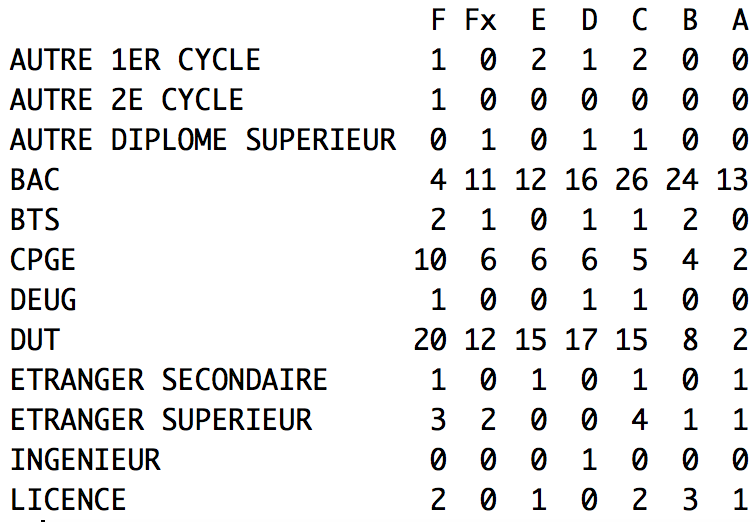
\includegraphics[width=0.65\linewidth]{img/1-1-2-Contingence-Result-Diplome-Origine}
		\caption{\scriptsize Tableau de contingence entre résultat et diplôme d'origine}
		\label{fig:tab_contingence_diplome_resultat}
	\end{subfigure}%
	\begin{subfigure}[b]{0.5\linewidth}
		\centering
		\captionsetup{justification=centering, margin=1cm}
		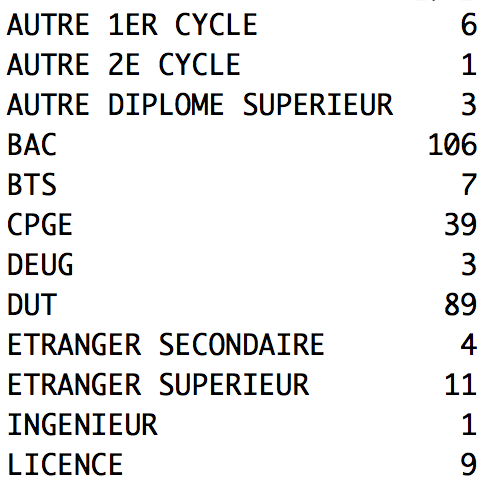
\includegraphics[width=0.5\linewidth]{img/1-1-2-Effectif-Diplome-Origine}
		\caption{\scriptsize Effectif total par diplôme}
		\label{fig:effectif_total_par_diplome}
	\end{subfigure}%
	\caption{
		\small Effectifs de la population par diplôme d'origine et tableau de contingence entre les variables \textit{résultat} et \textit{diplôme d'origine}.
	}
	\label{fig:tab_effectifs_et_contingence_resultats_diplome_origine}%
\end{figure}

On remarque immédiatement que les conditions du test ne sont pas respectées~: il a y une majorité des effectifs qui sont inférieurs à 5 dans le tableau de contingence  (\autoref{fig:tab_contingence_diplome_resultat}). Et c'est tout à fait normal si l'on regarde les effectifs d'étudiants (\autoref{fig:effectif_total_par_diplome}) en fonction de leur diplôme d'origine dans la population totale~: seuls les diplômes BAC (étudiant venant de tronc commun), DUT et CPGE sont convenablement représentés.
On peut tout de même effectuer le test du $\chi^2$ tout en sachant que les conditions ne sont pas respectées, afin de vérifier l'importance de ces conditions. On obtient alors une \textit{p-value} égale à $0.2572$, nous amenant à conserver l'hypothèse $H_{0}$ d'indépendance des variables, tout en sachant que le résultat est probablement faux.



\paragraph{Correction des effectifs}
Afin de respecter les conditions du test de $\chi^2$, nous n'avons gardé que les lignes correspondant aux diplômes d'origines de type \textit{BAC}, \textit{DUT} et \textit{CPGE}. Il a aussi fallut regrouper les deux premières et deux dernières classes de \textit{résultat} en sommant les effectifs des élèves ayant obtenu \textit{F} ou \textit{Fx} et ceux ayant eu \textit{A} ou \textit{B}.\\
On obtient ainsi un nouveau tableau de contingence~:


\begin{figure}[H]
	\centering
	\captionsetup{justification=centering, margin=4cm}
	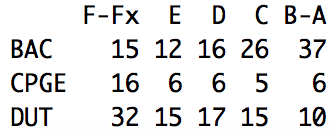
\includegraphics[width=0.3\linewidth]{img/1-1-2-Contingence-Result-Diplome-Corrigee}
	\caption{\scriptsize Tableau de contingence \textbf{corrigé} entre résultat et diplôme d'origine.}
	\label{fig:tab_effectifs_et_contingence_resultats_diplome_origine_corrigee}
\end{figure}
Les conditions du test sont alors réunies et on obtient une \textit{p-value} égale à $0.000288$. On rejette donc l'hypothèse $H_{0}$ d'indépendance avec confiance~: le diplôme d'origine d'un étudiant a un impact significatif sur son résultat final à l'UV de statistiques SY02.

Voici une représentation graphique de la fréquence des résultats en fonction du diplôme d'origine~:

\begin{figure}[H]
	\centering
	\captionsetup{justification=centering, margin=2cm}
	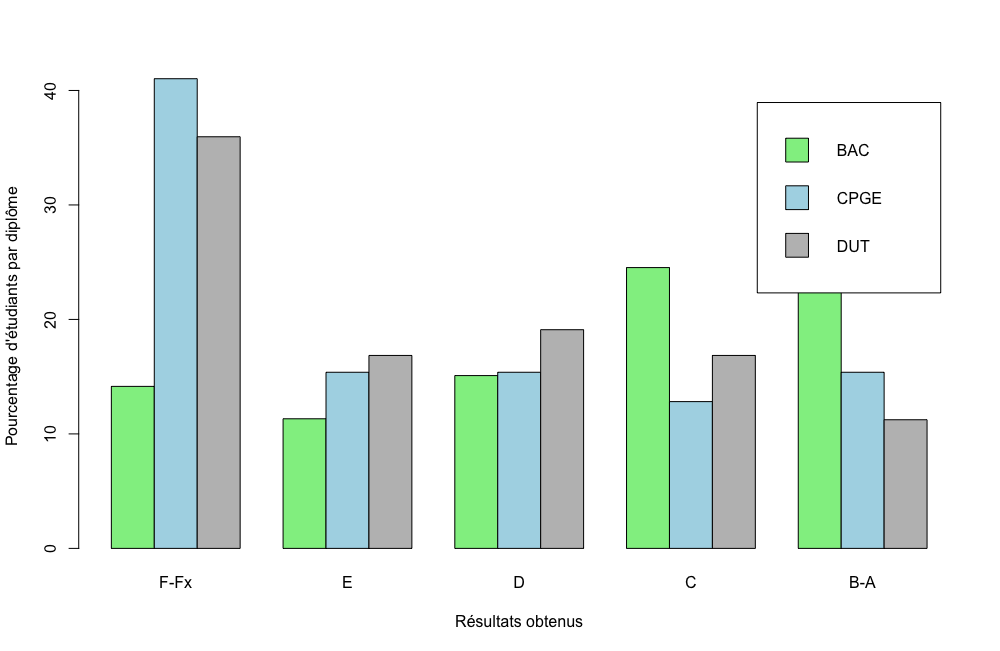
\includegraphics[width=.4\linewidth]{img/1-1-2-Ratio-resultat-diplome}
	\caption{\scriptsize Fréquence par diplôme d'origine et résultat}
	\label{fig:ratio_resultats_diplome}
\end{figure}


On remarque que 34\% des élèves ayant comme dernier diplôme le BAC ont obtenu \textit{A} ou \textit{B} tandis que seulement 14\% d'entre-eux n'ont pas réussi l'UV. On remarque aussi que la courbe est croissante~: plus le résultat est bon, plus la fréquence d'obtention augmente. C'est l'inverse pour les élèves provenant de DUT ou CPGE~: moins le résultat est bon, plus la fréquence d'élèves obtenant ce résultat augmente (environ 40\% des élèves en provenance d'un DUT ou de CPGE n'ont pas obtenu l'UV).


\subsubsection{Lien statistique entre le résultat et la spécialité des étudiants}

La spécialité des étudiants correspond à leur cursus actuel~: GB, GI, GM, GP, GSM, GSU, HuTech, ISS, ou TC. En s'intéressant à l'effectif de chaque classe, on remarque de suite qu'il va falloir en considérer quelques unes seulement pour respecter les conditions du test. Les classes telles que \textit{HuTech}, \textit{ISS}, \textit{TC} voire même \textit{GP} ne sont pas assez représentées pour être en mesure de respecter les conditions du tests d'indépendance du $\chi^2$.

\begin{figure}[H]
	\centering
	\captionsetup{justification=centering, margin=1cm}
	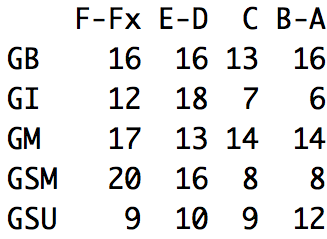
\includegraphics[width=0.2\linewidth]{img/1-1-2-Contingence-Result-Specialite-Corrige}
	\caption{\scriptsize Tableau de contingence \textbf{corrigé} entre résultat et spécialité}
	\label{fig:tab_contingence_diplome_specialite_corrige}
\end{figure}

Le test du $\chi^2$ effectué sur le tableau de contingence (voir \autoref{fig:tab_contingence_diplome_specialite_corrige}) donne une \textit{p-value} égale à 0.4673856. On accepte l'hypothèse $H_{0}$ d'indépendance des variables \textit{résultat} et \textit{spécialité} avec confiance.

Conclusion~: la spécialité d'un étudiant n'a pas d'impact sur son résultat.


\subsubsection{Lien statistique entre le résultat et le niveau des étudiants}

Le niveau des étudiants correspond à leur semestre actuel de branche, de 1 à 6 (deux semestres par an sur un cursus de trois ans).

\begin{figure}[H]
	\centering
	\captionsetup{justification=centering, margin=1cm}
	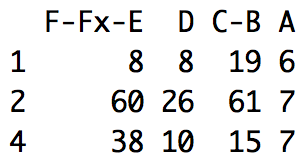
\includegraphics[width=0.2\linewidth]{img/1-1-2-Contingence-Result-Niveau-Corrige}
	\caption{\scriptsize Tableau de contingence \textbf{corrigé} entre résultat et niveau}
	\label{fig:tab_contingence_diplome_niveau_corrige}
\end{figure}

Le test du $\chi^2$ effectué sur le tableau de contingence \ref{fig:tab_contingence_diplome_niveau_corrige} donne une \textit{p-value} égale à 0.003523739. On réfute l'hypothèse $H_{0}$ d'indépendance des variables \textit{résultat} et \textit{niveau}.

Conclusion~: le niveau d'un étudiant impacte son résultat. On observe par exemple dans la figure \ref{fig:frequence_resultats_niveau} que plus le niveau de l'étudiant augmente, moins il a de chance d'obtenir l'UV. 42\% de \textit{F} ou \textit{Fx} pour les étudiants de niveau 4 contre 7\% seulement pour ceux de niveau 1. A l'opposé, ces derniers sont 80\% à obtenir l'UV avec un résultat entre \textit{D} et \textit{A} contre 45\% pour les étudiants de niveau 4. Les étudiants de niveau 2 se situent au milieu, avec 60\% pour un résultat compris entre \textit{D} et \textit{A} et 27\% de non obtention de l'UV.

\begin{figure}[H]
	\centering
	\captionsetup{justification=centering, margin=2cm}
	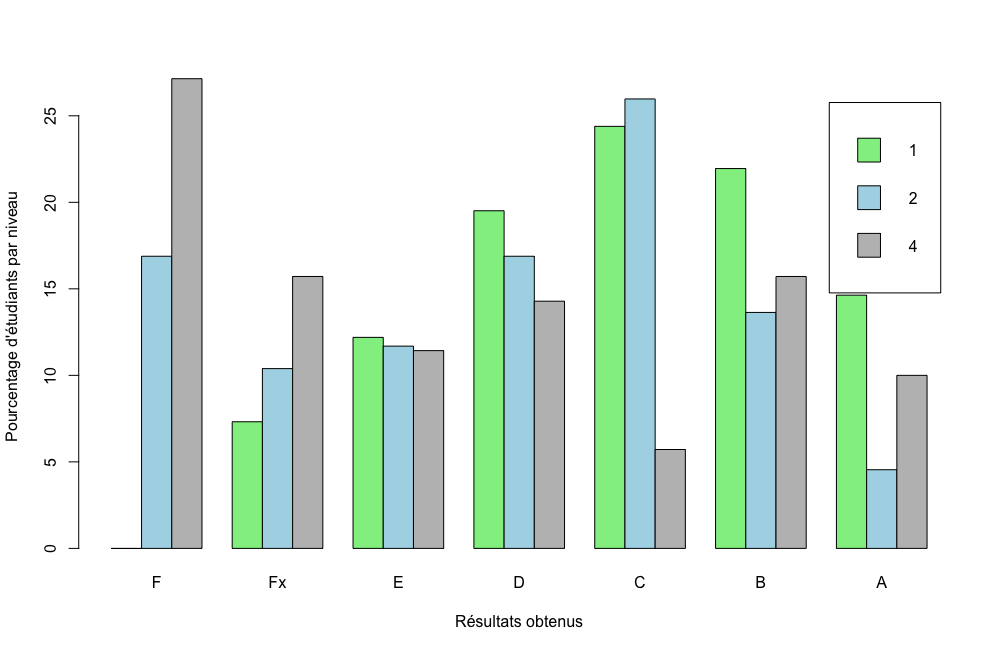
\includegraphics[width=.5\linewidth]{img/1-1-2-Ratio-resultat-niveau}
	\caption{\scriptsize Fréquence d'obtention d'un résultat en fonction du niveau de l'étudiant}
	\label{fig:frequence_resultats_niveau}
\end{figure}

\subsubsection{Lien statistique entre le résultat et les correcteurs}

Selon toute vraisemblance, le correcteur ne devrait pas influer sur le résultat d'un étudiant à l'UV. Nous allons tout de même nous en assurer. Le principe est le même que précédemment~: construire le tableau de contingence, regrouper des classes au besoin pour respecter les conditions du test du $\chi^2$ et effectuer ce test afin de déterminer si les variables sont indépendantes ou non.


Le test du $\chi^2$ effectué sur le tableau de contingence \textit{notes médian} / \textit{correcteurs médian} (voir \autoref{fig:contingence_resultats_correcteur_corrige}) donne une \textit{p-value} égale à 0.499. On conserve donc l'hypothèse $H_{0}$ d'indépendance.
\\Le même principe a été appliqué sur le couple de variables \textit{note final} et \textit{correcteur final} à la différence qu'il y a trois classes au lieu de 4 afin de respecter les conditions du test. La \textit{p-value} obtenue vaut 0.115. On conserve là aussi l'hypothèse $H_{0}$ d'indépendance.


\begin{figure}[H]
	\centering
	\captionsetup{justification=centering, margin=4cm}
	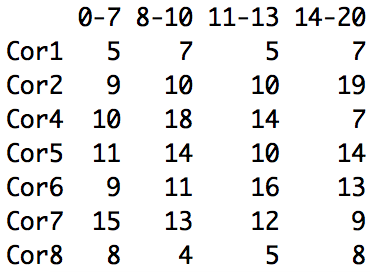
\includegraphics[width=.2\linewidth]{img/1-1-2-Contingence-Result-Correcteur-Median-Corrige}
	\caption{\scriptsize Tableau de contingence \textbf{après regroupement} entre les notes du médian et les correcteurs}
	\label{fig:contingence_resultats_correcteur_corrige}
\end{figure}



Les notes du médian et du final étant fortement corrélées au résultat obtenu (\autoref{fig:boxplot_note_resultat}), on peut conclure en affirmant que les variables \textit{correcteur} et \textit{résultat} sont indépendantes.

\begin{figure}[H]
	\centering
	\captionsetup{justification=centering, margin=4cm}
	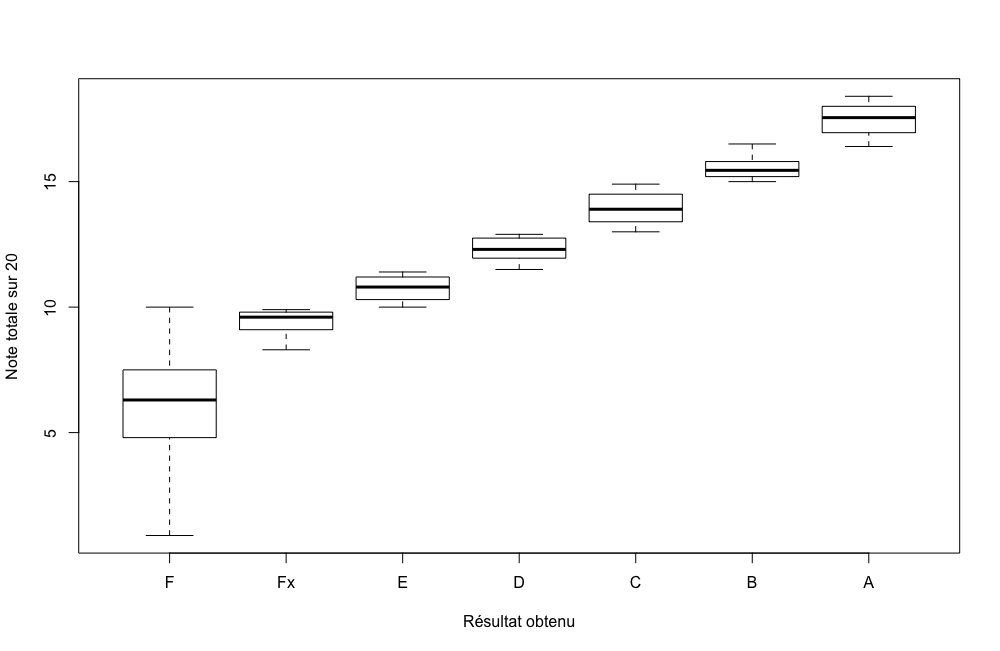
\includegraphics[width=.5\linewidth]{img/1-1-2-Boxplot-note-resultat}
	\caption{\scriptsize Distribution des résultats obtenus en fonction de la note finale}
	\label{fig:boxplot_note_resultat}
\end{figure}

\section{Données Crabs}

\subsection{Analyse descriptive}

\subsubsection{Description des données}
\label{subsection:describe_crabs}

Le jeu de données présente 200 crabes classés en fonction de leur espèce et de leur sexe. Chaque individu est aussi décrit par 5 caractéristiques morphologiques quantitatives.
\\
Liste des variables qualitatives~:
\begin{itemize}
	\item \textbf{sex}~: le sexe du crabe, \textit{M} pour mâle, \textit{F} pour femelle.
	\item \textbf{sp}~: espèce à laquelle appartient un individu, \textit{O} pour \textit{Orange}, \textit{B} pour \textit{Bleu}.
\end{itemize}
Liste des variables quantitatives~:
\begin{itemize}
	\item \textbf{FL}~: taille de la frontale.
	\item \textbf{RW}~: largeur de la queue.
	\item \textbf{CL}~: longueur de la coquille.
	\item \textbf{CW}~: largeur de la coque.
	\item \textbf{BD}~: la profondeur du corps.
\end{itemize}
Il existe aussi une autre variable numérique, purement utilitaire, qui est l'index~:
\begin{itemize}
	\item \textbf{[1-50]}~: mâles d'espèce bleue.
	\item \textbf{[51-100]}~: femelles d'espèce bleue.
	\item \textbf{[101-150]}~: mâles d'espèce orange.
	\item \textbf{[151-200]}~: femelles d'espèce orange.
\end{itemize}


\subsubsection{Données morphologiques}

Les deux figures suivantes présentent les distributions des variables morphologiques en fonction de l'espèce (\autoref{fig:morphemetriques_en_fonction_espece}) et du sexe (\autoref{fig:morphemetriques_en_fonction_sexe}).\\


\begin{figure}[H]
	\centering
	\captionsetup{justification=centering, margin=2cm}
	\begin{subfigure}[b]{0.3\linewidth}
		\centering
		\captionsetup{justification=centering, margin=1cm}
		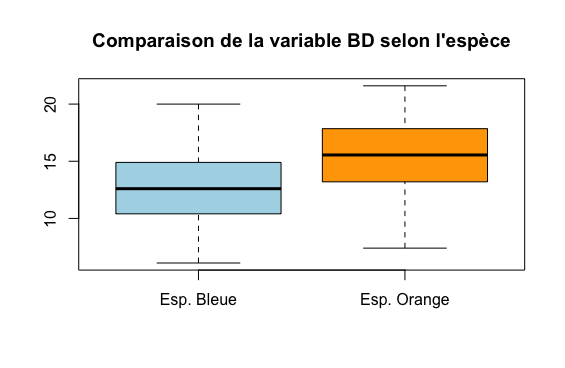
\includegraphics[width=1\linewidth]{img/1-2-1-espece-bd.png}
		\caption{\scriptsize Variable BD}
		\label{fig:1_2_1_espece_bd}
	\end{subfigure}%
	\begin{subfigure}[b]{0.3\linewidth}
		\centering
		\captionsetup{justification=centering, margin=1cm}
		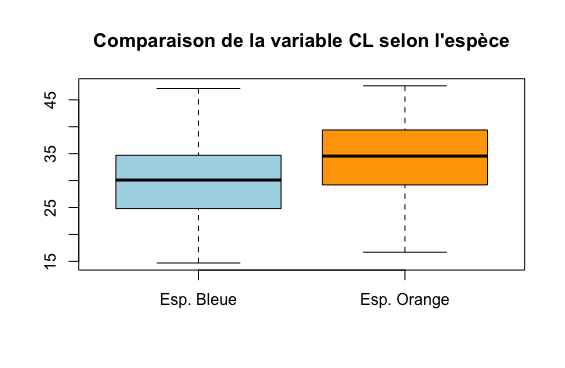
\includegraphics[width=1\linewidth]{img/1-2-1-espece-cl.png}
		\caption{\scriptsize Variable CL}
		\label{fig:1_2_1_espece_cl}
	\end{subfigure}%
	\begin{subfigure}[b]{0.3\linewidth}
		\centering
		\captionsetup{justification=centering, margin=1cm}
		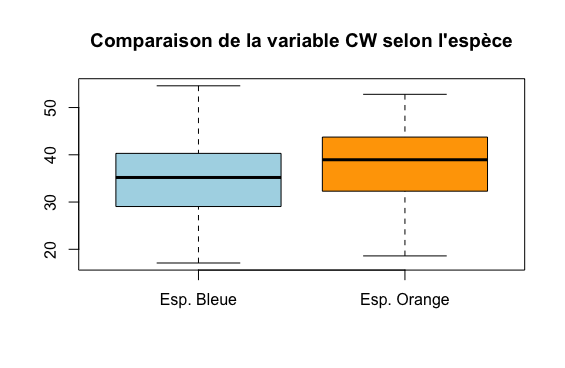
\includegraphics[width=1\linewidth]{img/1-2-1-espece-cw.png}
		\caption{\scriptsize Variable CW}
		\label{fig:1_2_1_espece_cw}
	\end{subfigure}%
	\\
	\begin{subfigure}[b]{0.3\linewidth}
		\centering
		\captionsetup{justification=centering, margin=1cm}
		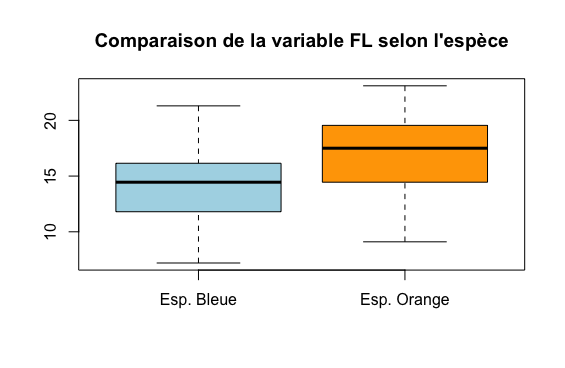
\includegraphics[width=1\linewidth]{img/1-2-1-espece-fl.png}
		\caption{\scriptsize Variable FL}
		\label{fig:1_2_1_espece_fl}
	\end{subfigure}%
	\begin{subfigure}[b]{0.3\linewidth}
		\centering
		\captionsetup{justification=centering, margin=1cm}
		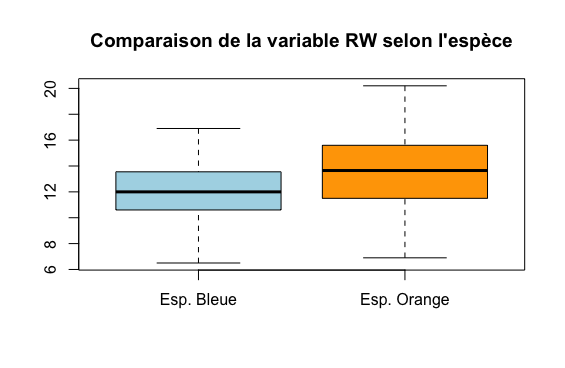
\includegraphics[width=1\linewidth]{img/1-2-1-espece-rw.png}
		\caption{\scriptsize Variable RW}
		\label{fig:1_2_1_espece_rw}
	\end{subfigure}%
	\caption{
		\small Distributions des variables morphométriques en fonction de l'espèce.
	}
	\label{fig:morphemetriques_en_fonction_espece}%
\end{figure}%

\begin{figure}[H]
	\centering
	\captionsetup{justification=centering, margin=2cm}
	\begin{subfigure}[b]{0.3\linewidth}
		\centering
		\captionsetup{justification=centering, margin=1cm}
		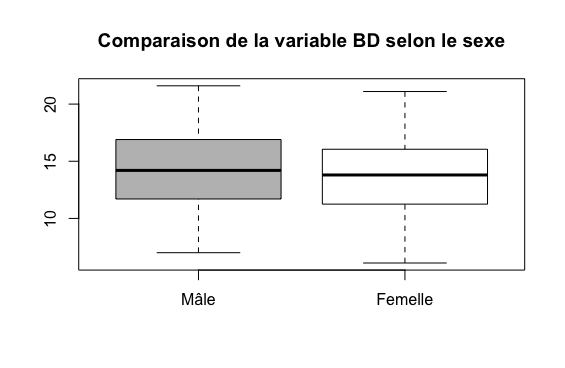
\includegraphics[width=1\linewidth]{img/1-2-1-sex-bd.png}
		\caption{\scriptsize Variable BD}
		\label{fig:1_2_1_sex_bd}
	\end{subfigure}%
	\begin{subfigure}[b]{0.3\linewidth}
		\centering
		\captionsetup{justification=centering, margin=1cm}
		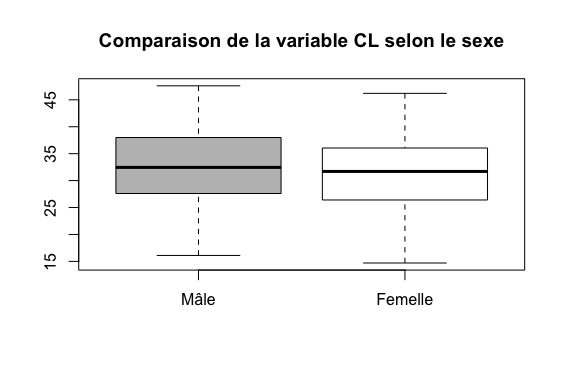
\includegraphics[width=1\linewidth]{img/1-2-1-sex-cl.png}
		\caption{\scriptsize Variable CL}
		\label{fig:1_2_1_sex_cl}
	\end{subfigure}%
	\begin{subfigure}[b]{0.3\linewidth}
		\centering
		\captionsetup{justification=centering, margin=1cm}
		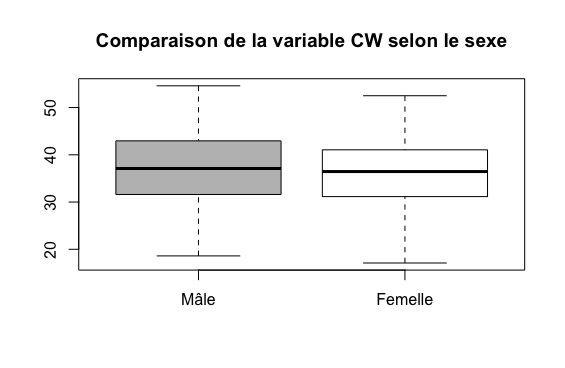
\includegraphics[width=1\linewidth]{img/1-2-1-sex-cw.png}
		\caption{\scriptsize Variable CW}
		\label{fig:1_2_1_sex_cw}
	\end{subfigure}%
	\\
	\begin{subfigure}[b]{0.3\linewidth}
		\centering
		\captionsetup{justification=centering, margin=1cm}
		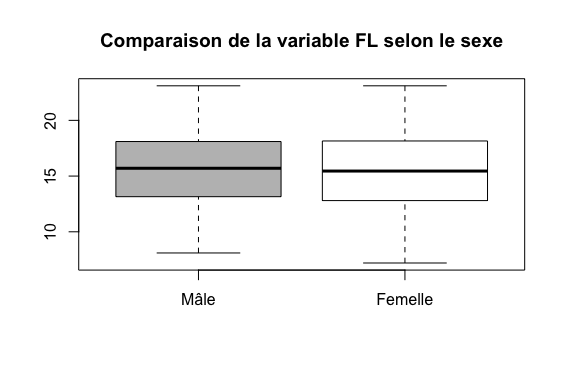
\includegraphics[width=1\linewidth]{img/1-2-1-sex-fl.png}
		\caption{\scriptsize Variable FL}
		\label{fig:1_2_1_sex_fl}
	\end{subfigure}%
	\begin{subfigure}[b]{0.3\linewidth}
		\centering
		\captionsetup{justification=centering, margin=1cm}
		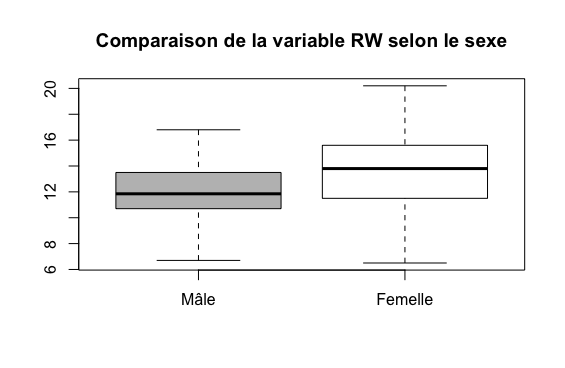
\includegraphics[width=1\linewidth]{img/1-2-1-sex-rw.png}
		\caption{\scriptsize Variable RW}
		\label{fig:1_2_1_sex_rw}
	\end{subfigure}%
	\caption{
		\small Distributions des variables morphométriques en fonction du sexe.
	}
	\label{fig:morphemetriques_en_fonction_sexe}%
\end{figure}

Graphiquement, il semble difficile de séparer les individus en fonction de leur sexe ou de leur espèce. Comparer les populations de même sexe mais d'espèce différente, de même espèce mais de sexe différent ou encore de sexe et espèce différents donne des résultats similaires. Aucune de ces variables, prise individuellement, ne nous permet d'identifier le sexe ou l'espèce d'un individu.

\subsection{Etude de la corrélation entre les variables morphologiques}
\label{subsection:crabs_correlation_variables_quantitatives}

La corrélation entre les cinq variables est très forte, comme le montre le tableau de corrélation suivant~:
\begin{table}[h]
	\centering
	\captionsetup{justification=centering, margin=2cm}
	\caption{Corrélations entre les variables quantitatives de la population de crabes.}
	\begin{tabular}{r|rrrrr}
		& FL & RW & CL & CW & BD \\ 
		\hline
		FL & 1.00 & 0.91 & 0.98 & 0.96 & 0.99 \\ 
		RW & 0.91 & 1.00 & 0.89 & 0.90 & 0.89 \\ 
		CL & 0.98 & 0.89 & 1.00 & 1.00 & 0.98 \\ 
		CW & 0.96 & 0.90 & 1.00 & 1.00 & 0.97 \\ 
		BD & 0.99 & 0.89 & 0.98 & 0.97 & 1.00 \\ 
	\end{tabular}
\end{table}

De plus, toutes les variables sont corrélées positivement entre-elles. La raison est simple~: les observations représentent des mesures morphométriques, c'est à dire des distances relevées sur les corps des crabes. Plus un crabe est grand, plus ces mesures vont grandir, et inversement.
Pour s'affranchir de ce phénomène, on pourra pratiquer une analyse en composantes principales sur les données. Les nouvelles composantes identifiées devraient présenter une faible corrélation entre elles. Il sera alors peut-être possible de différencier le sexe et l'espèce des individus en fonction de leur mesures morphométriques (voir \autoref{sec:2_3_ACP_Crabs}).


\section{Données Pima}
\label{section:pima-descriptif}

Les données Pima consistent en plusieurs mesures effectuées sur une population de femmes amérindiennes, le but étant d'observer les facteurs aggravant le diabète dans une population plus touchée que la moyenne par cette maladie.
L'échantillon est composé 532 individus décrits par 8 variables différentes, toutes quantitatives sauf une qui détermine l'absence ou la présence de diabète chez l'individu.

\subsection{Analyse descriptive}

\subsubsection{Liste des variables}

Variables quantitatives~:
\begin{itemize}
	\item \textbf{npreg}~: nombre de grossesses.
	\item \textbf{glu}~: taux plasmatique de glucose.
	\item \textbf{bp}~: pression artérielle diastolique.
	\item \textbf{skin}~: épaisseur du pli cutané au niveau du triceps.
	\item \textbf{bmi}~: indice de masse corporelle.
	\item \textbf{ped}~: fonction de pedigree du diabète, c'est à dire une mesure de l’influence génétique espérée des proches, affectés ou non par le diabète, sur le risque éventuel du sujet.
	\item \textbf{age}~: l'age du sujet.
\end{itemize}
Variable qualitative~:
\begin{itemize}
	\item \textbf{z}~: diabétique si \textbf{z} = 2.
\end{itemize}

\subsubsection{Domaine de définition des variables}

\begin{table}[H]
	\centering
	\captionsetup{justification=centering, margin=2cm}
	\caption{Résumé des variables composant le jeu de données \texttt{Pima}.}
	\begin{tabular}{|l|l|l|l|l}
		\hline
		npreg &      glu &       bp &      skin &      bmi \\
		\hline
		Min.   : 0.000   & Min.   : 56.00   & Min.   : 24.00   & Min.   : 7.00   & Min.   :18.20  \\
		1st Qu.: 1.000   & 1st Qu.: 98.75   & 1st Qu.: 64.00   & 1st Qu.:22.00   & 1st   Qu.:27.88  \\
		Median : 2.000   & Median :115.00   & Median : 72.00   & Median :29.00   & Median :32.80  \\
		Mean   : 3.517   & Mean   :121.03   & Mean   : 71.51   & Mean   :29.18   & Mean  :32.89  \\ 
		3rd Qu.: 5.000   & 3rd Qu.:141.25   & 3rd Qu.: 80.00   & 3rd Qu.:36.00   & 3rd Qu.:36.90  \\
		Max.   :17.000   & Max.   :199.00   & Max.   :110.00   & Max.   :99.00   & Max.   :67.10  \\
	\end{tabular}
	\begin{tabular}{l|l|l|}
		\hline
		ped &      age & z \\ 
		\hline
		Min.   :0.0850   & Min.   :21.00   & 1:355   \\ 
		1st Qu.:0.2587   & 1st Qu.:23.00   & 2:177   \\ 
		Median :0.4160   & Median :28.00   &  \\ 
		Mean   :0.5030   & Mean   :31.61   &  \\ 
		3rd Qu.:0.6585   & 3rd Qu.:38.00   &  \\ 
		Max.   :2.4200   & Max.   :81.00   &  \\ 
	\end{tabular}
\end{table}


La première chose importante que nous remarquons est la différence d'effectif entre les types d'individus~: il y a deux fois plus d'individus non diabétiques (355) que de diabétiques (177). Le choix des représentations graphiques et tests statistiques est alors important. Travailler sur l'effectif simple avec par exemple des diagrammes en bâton donnera des résultat complètement faux. Des boîtes à moustache par contre seront plus à même de pointer des disparités entre les deux groupes d'individus.


\paragraph{Corrélation entre les variables quantitatives}

Cette étude de la corrélation (voir \autoref{table:correlation-quant-pima}), sans prendre en compte le facteur diabète, ne nous apprend pas grand chose sinon que les variables sont peu corrélées entre-elles, mise à part l'âge et la grossesse. Ces deux dernières sont légèrement corrélées positivement~: plus la femme interrogée est âgé, plus il y a de chance qu'elle ait eu plusieurs grossesses dans sa vie.


\begin{table}[H]
	\centering
	\captionsetup{justification=centering, margin=4cm}
	\caption{Corrélations entre les variables quantitatives du jeu de données \texttt{Pima}.}
	\begin{tabular}{r|rrrrrrr}
		& npreg & glu & bp & skin & bmi & ped & age \\ 
		\hline
		npreg & 1.000 & 0.125 & 0.205 & 0.095 & 0.009 & 0.007 & 0.641 \\ 
		glu & 0.125 & 1.000 & 0.219 & 0.227 & 0.247 & 0.166 & 0.279 \\ 
		bp & 0.205 & 0.219 & 1.000 & 0.226 & 0.307 & 0.008 & 0.347 \\ 
		skin & 0.095 & 0.227 & 0.226 & 1.000 & 0.647 & 0.119 & 0.161 \\ 
		bmi & 0.009 & 0.247 & 0.307 & 0.647 & 1.000 & 0.151 & 0.073 \\ 
		ped & 0.007 & 0.166 & 0.008 & 0.119 & 0.151 & 1.000 & 0.072 \\ 
		age & 0.641 & 0.279 & 0.347 & 0.161 & 0.073 & 0.072 & 1.000 \\ 
	\end{tabular}
	\label{table:correlation-quant-pima}
\end{table}


\subsection{Etude des liens statistique entre le facteur diabète \textit{z} et les autres variables}

Pour étudier les liens statistiques entre le facteur diabète et les autres variables, voici la procédure que nous allons suivre~:
\begin{itemize}
	\item Effectuer des représentations de boîte à moustache de l'ensemble des variables en fonction du facteur diabète.
	\item Valider statistiquement les observations graphiques avec un test du $\chi^2$ effectué sur le tableau de contingence correspondant au couple de variable ( et vérifiant les conditions du test).
	\item Représenter graphiquement le tableau de fréquence afin d'avoir une vision graphique de l'influence (ou de la non influence) du facteur diabète sur la variable étudiée. Le tableau de fréquence correspond au tableau de contingence exprimé en pourcentage de représentation d'une valeur par rapport à la population totale du groupe (diabétique / non diabétique) à laquelle elle appartient.
\end{itemize}

Note : la couleur verte représente la population non diabétique, la couleur bleu les individus souffrant de diabète. 

\subsubsection{Représentation des variables en fonction du facteur diabète}

\begin{figure}[H]
	\centering
	\captionsetup{justification=centering, margin=2cm}
	\begin{subfigure}[b]{0.25\linewidth}
		\centering
		\captionsetup{justification=centering}
		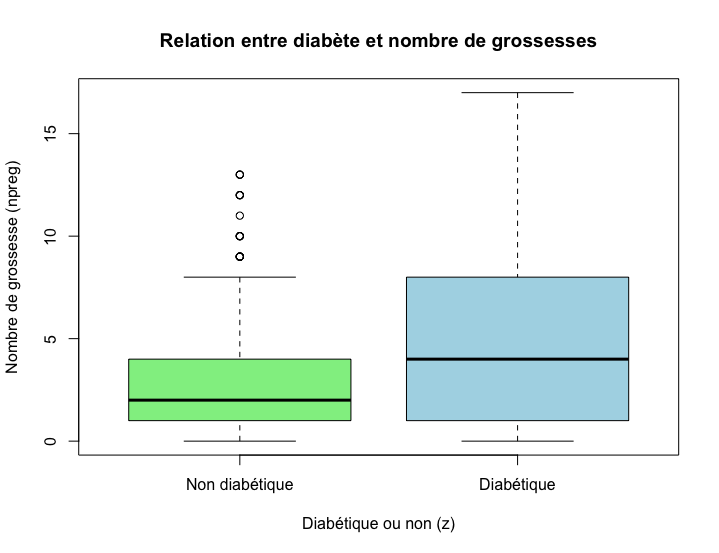
\includegraphics[width=1\linewidth]{img/1-3-2-boxplot-diabete-grossesses}
		\caption{\scriptsize Nombre de grossesses}
		\label{fig:1-3-2-boxplot-diabete-grossesses}
	\end{subfigure}%
	\begin{subfigure}[b]{0.25\linewidth}
		\centering
		\captionsetup{justification=centering}
		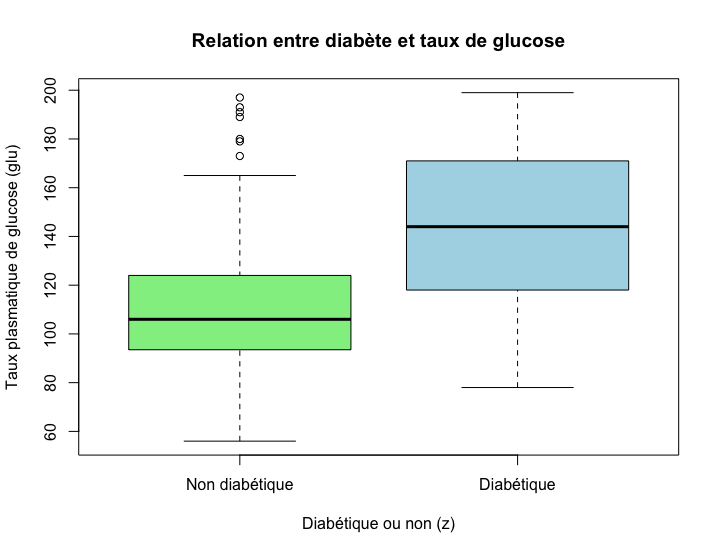
\includegraphics[width=1\linewidth]{img/1-3-2-boxplot-diabete-glucose}
		\caption{\scriptsize Taux de glucose}
		\label{fig:1-3-2-boxplot-diabete-glucose}
	\end{subfigure}%
	\begin{subfigure}[b]{0.25\linewidth}
		\centering
		\captionsetup{justification=centering}
		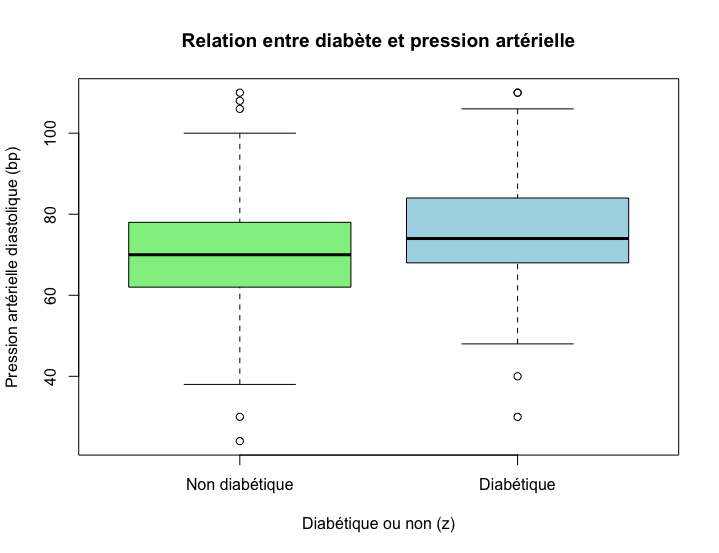
\includegraphics[width=1\linewidth]{img/1-3-2-boxplot-diabete-pression-arterielle}
		\caption{\scriptsize Pression artérielle}
		\label{fig:1-3-2-boxplot-diabete-pression-arterielle}
	\end{subfigure}%
	\begin{subfigure}[b]{0.25\linewidth}
		\centering
		\captionsetup{justification=centering}
		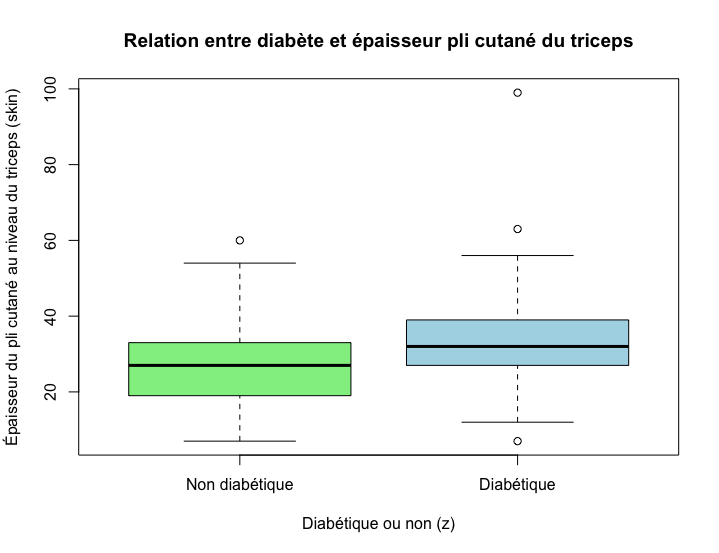
\includegraphics[width=1\linewidth]{img/1-3-2-boxplot-diabete-pli-cutane}
		\caption{\scriptsize Epaisseur pli cutané}
		\label{fig:1-3-2-boxplot-diabete-pli-cutane}
	\end{subfigure}%
	\\
	\begin{subfigure}[b]{0.25\linewidth}
		\centering
		\captionsetup{justification=centering}
		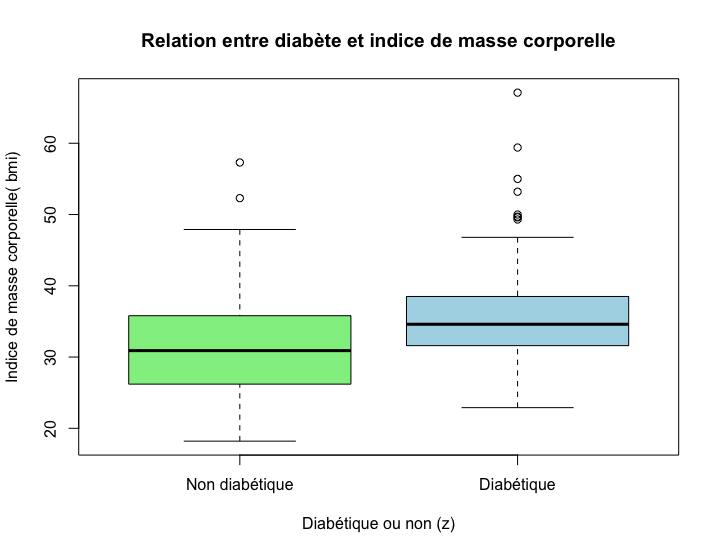
\includegraphics[width=1\linewidth]{img/1-3-2-boxplot-diabete-indice-masse-corp}
		\caption{\scriptsize Indice de masse corp.}
		\label{fig:1-3-2-boxplot-diabete-indice-masse-corp}
	\end{subfigure}%
	\begin{subfigure}[b]{0.25\linewidth}
		\centering
		\captionsetup{justification=centering}
		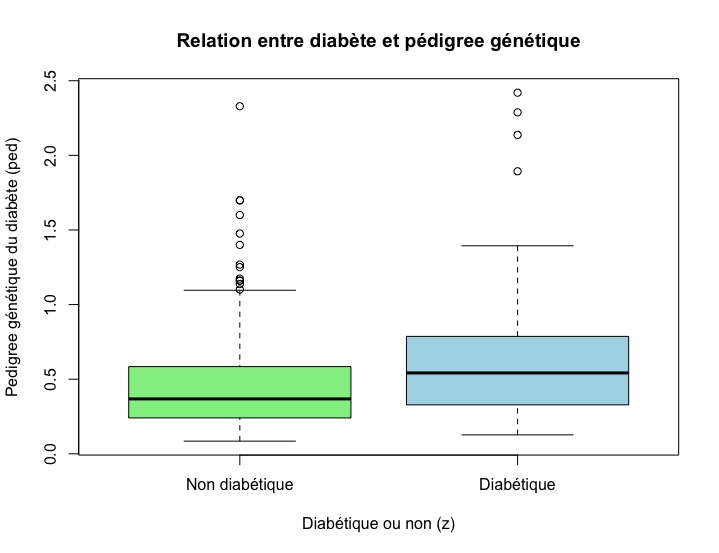
\includegraphics[width=1\linewidth]{img/1-3-2-boxplot-diabete-pedigree}
		\caption{\scriptsize Pedigree génétique}
		\label{fig:1-3-2-boxplot-diabete-pedigree}
	\end{subfigure}%
	\begin{subfigure}[b]{0.25\linewidth}
		\centering
		\captionsetup{justification=centering}
		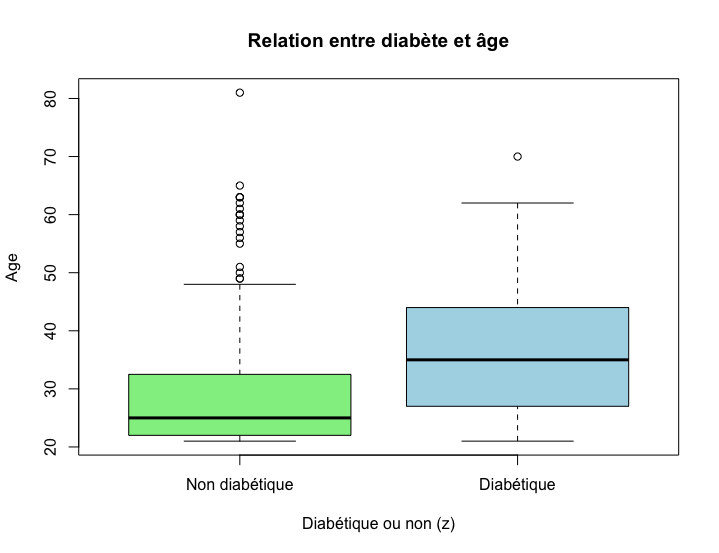
\includegraphics[width=1\linewidth]{img/1-3-2-boxplot-diabete-age}
		\caption{\scriptsize Age}
		\label{fig:1-3-2-boxplot-diabete-age}
	\end{subfigure}%
	\caption{
		\small Distributions des variables en fonction du diabète.
	}
	\label{fig:box_plot_diabete_pima}%
\end{figure}




Visuellement, il semblerait que le facteur diabète soit lié à l'âge, au nombre de grossesses et au taux de glucose dans le sang. Les quatre autres variables ne semblent pas diverger de façon remarquable en fonction du diabète, même si quelques différences sont déjà notables.



\subsubsection{Tests du $\chi^2$ d'indépendance des variables}

\begin{itemize}
	\item \textbf{Diabète vs. Nombre de grossesses}
	\\ \textit{p-value} = 2.215e-08
	\\ Conclusion~: les variables ne sont pas indépendantes.
	
	\item \textbf{Diabète vs. Taux plasmatique de glucose}
	\\ \textit{p-value} < 2.2e-16
	\\ Conclusion~: les variables ne sont pas indépendantes, et c'est tout à fait logique, le diabète étant une maladie où le manque d'insuline \textthreequartersemdash\ hormone en charge de la régulation du glucose \textthreequartersemdash\ cause une élévation anormale du taux de ce dernier.
	
	\item \textbf{Diabète vs. Pression artérielle diastolique}
	\\ \textit{p-value} = 0.0001862
	\\ Conclusion~: les variables ne sont pas indépendantes.
	
	\item \textbf{Diabète vs. Epaisseur du pli cutané au niveau du triceps}
	\\ \textit{p-value} = 9.256e-06
	\\ Conclusion~: les variables ne sont pas indépendantes.
	
	\item \textbf{Diabète vs. Indice de masse corporelle}
	\\ \textit{p-value} = 3.476e-11
	\\ Conclusion~: les variables ne sont pas indépendantes.
	
	\item \textbf{Diabète vs. Fonction de pedigree génétique du diabète}
	\\ \textit{p-value} = 1.65e-05
	\\ Conclusion~: les variables ne sont pas indépendantes.
	
	\item \textbf{Diabète vs. Age}
	\\ \textit{p-value} = 9.442e-14
	\\ Conclusion~: les variables ne sont pas indépendantes.
\end{itemize}


Contrairement à ce qu'on pensait précédemment, on se rend compte que toutes les variables sont plus ou moins influencées par le facteur diabète. Pour certaines, comme le taux de glucose, cela se comprend facilement. Pour d'autres, l'explication ne nous est pas connue. Nous allons par la suite représenter graphiquement les tableaux de fréquence afin de comprendre l'effet du diabète sur ces variables et inversement.

\subsubsection{Représentation graphique des tableaux de fréquence en fonction du facteur diabète}


\begin{figure}[H]
	\centering
	\captionsetup{justification=centering, margin=2cm}
	\begin{subfigure}[b]{0.25\linewidth}
		\centering
		\captionsetup{justification=centering}
		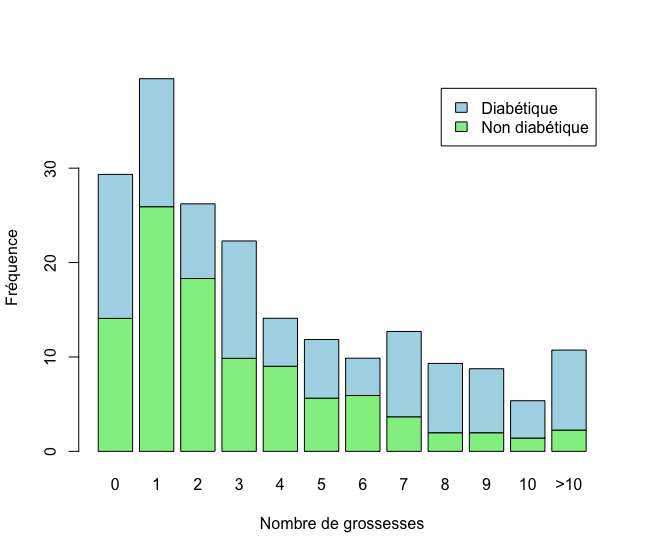
\includegraphics[width=1\linewidth]{img/1-3-2-barplot-freq-diabete-grossesses}
		\caption{\scriptsize Nombre de grossesses}
		\label{fig:1-3-2-barplot-freq-diabete-grossesses}
	\end{subfigure}%
	\begin{subfigure}[b]{0.25\linewidth}
		\centering
		\captionsetup{justification=centering}
		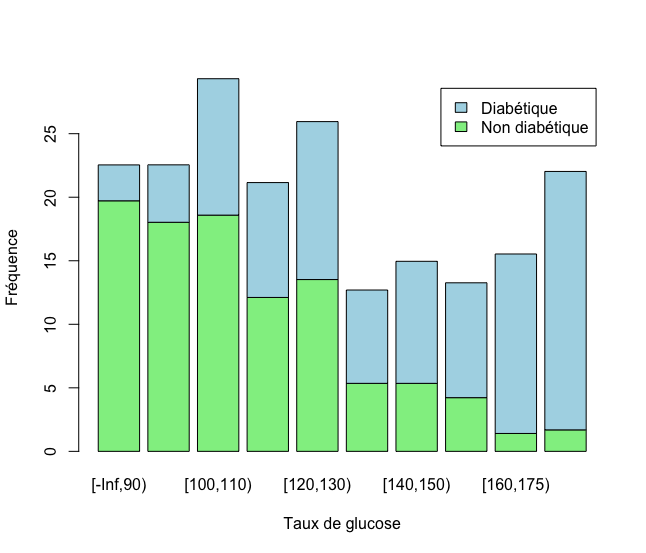
\includegraphics[width=1\linewidth]{img/1-3-2-barplot-freq-diabete-glucose}
		\caption{\scriptsize Taux de glucose}
		\label{fig:1-3-2-barplot-freq-diabete-glucose}
	\end{subfigure}%
	\begin{subfigure}[b]{0.25\linewidth}
		\centering
		\captionsetup{justification=centering}
		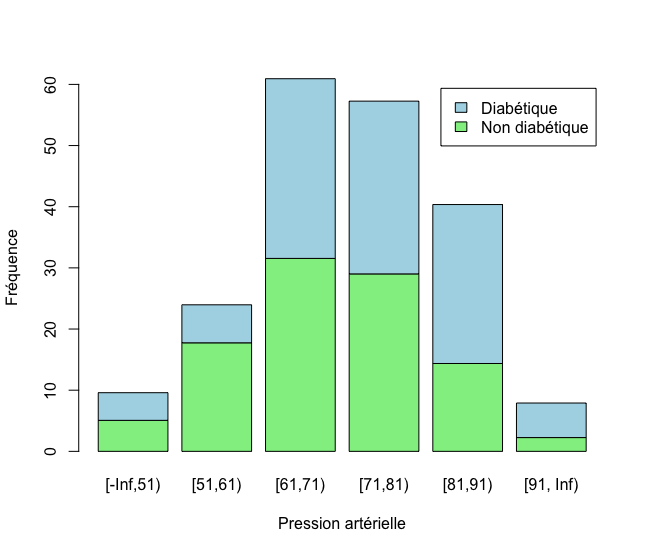
\includegraphics[width=1\linewidth]{img/1-3-2-barplot-freq-diabete-pression-arterielle}
		\caption{\scriptsize Pression artérielle}
		\label{fig:1-3-2-barplot-freq-diabete-pression-arterielle}
	\end{subfigure}%
	\begin{subfigure}[b]{0.25\linewidth}
		\centering
		\captionsetup{justification=centering}
		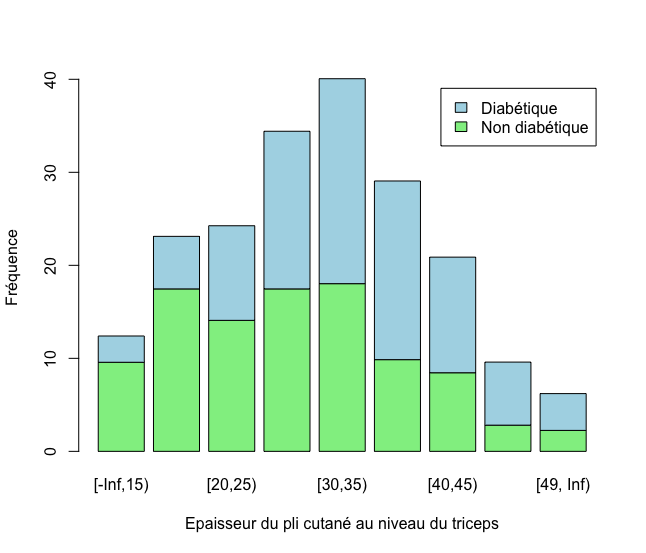
\includegraphics[width=1\linewidth]{img/1-3-2-barplot-freq-diabete-pli-cutane}
		\caption{\scriptsize Epaisseur pli cutané}
		\label{fig:1-3-2-barplot-freq-diabete-pli-cutane}
	\end{subfigure}%
	\\
	\begin{subfigure}[b]{0.25\linewidth}
		\centering
		\captionsetup{justification=centering}
		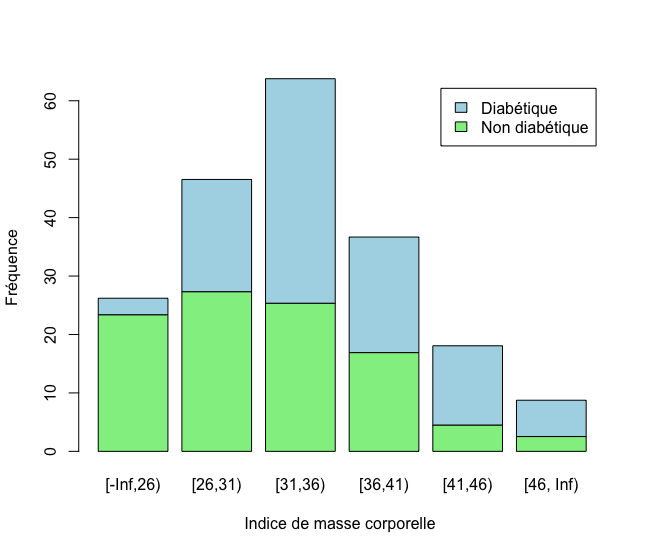
\includegraphics[width=1\linewidth]{img/1-3-2-barplot-freq-diabete-ind-masse-corp}
		\caption{\scriptsize Indice de masse corp.}
		\label{fig:1-3-2-barplot-freq-diabete-ind-masse-corp}
	\end{subfigure}%
	\begin{subfigure}[b]{0.25\linewidth}
		\centering
		\captionsetup{justification=centering}
		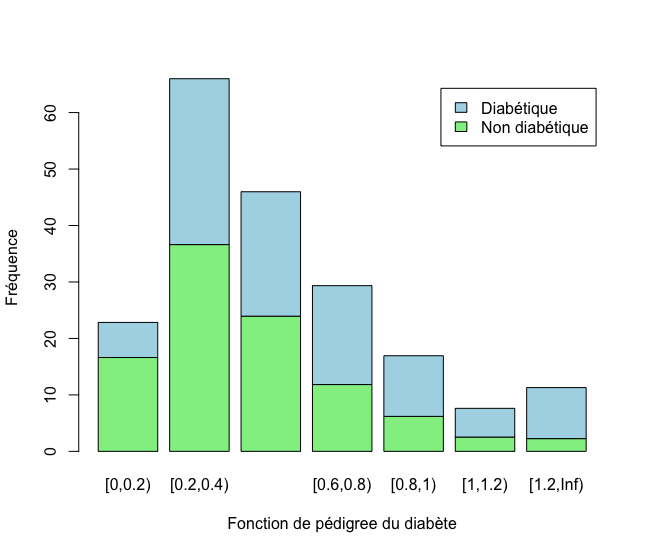
\includegraphics[width=1\linewidth]{img/1-3-2-barplot-freq-diabete-pedigree}
		\caption{\scriptsize Pedigree génétique}
		\label{fig:1-3-2-barplot-freq-diabete-pedigree}
	\end{subfigure}%
	\begin{subfigure}[b]{0.25\linewidth}
		\centering
		\captionsetup{justification=centering}
		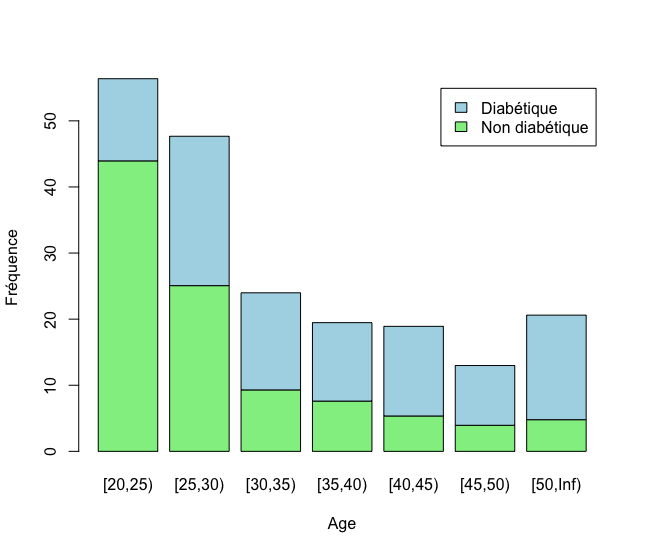
\includegraphics[width=1\linewidth]{img/1-3-2-barplot-freq-diabete-age}
		\caption{\scriptsize Age}
		\label{fig:1-3-2-barplot-freq-diabete-age}
	\end{subfigure}%
	\caption{
		\small Fréquences observées en fonction du facteur diabète.
	}
	\label{fig:bar_plot_freq_diabete_pima}%
\end{figure}


Rappel~: vert = non\ diabétique ; bleu = diabétique.

Ces graphiques nous donnent deux informations~: la fréquence d'observation au sein d'une population diabétique ou non diabétique, mais aussi la différence de fréquence entre ces deux populations. C'est à notre sens cette deuxième information qui est la plus importante si on veut comprendre l'impact du facteur diabète sur les variables.

\subsubsection{Analyses de l'interdépendance entre le diabète et les autres variables}

\begin{itemize}
	\item \textbf{Diabète vs. Nombre de grossesses}
	\\ Pour un nombre de grossesses inférieur à 7, la différence de fréquence entre les deux populations n'est pas flagrante mais tends à défavoriser l'apparition de diabète. Par contre, à partir de 7 grossesses et plus, il y a une écrasante majorité d'individus atteints de diabète. Le fait d'être enceinte ou pas nous paraissant indépendant du diabète, notre conclusion est que c'est un nombre répété de grossesses qui va favoriser l'apparition du diabète (et non pas le diabète qui induit un nombre élevé de grossesses).
		
	\item \textbf{Diabète vs. Taux plasmatique de glucose}
	\\ Comme dit précédemment, le manque d'insuline dans le corps implique une élévation du taux de glucose dans le sang. On peut dire que ce taux de glucose est un facteur indicatif de la présence ou de l'absence d'une condition diabétique.
		
	\item \textbf{Diabète vs. Pression artérielle diastolique}
	\\ Ces deux facteurs sont liés, mais assez faiblement. Les individus diabétiques ont une légère tendance à avoir une pression artérielle plus élevée que les non diabétiques. Nous n'avons pas d'explication causale, à savoir si c'est le diabète qui favorise l'hypertension (et pourquoi) ou bien si c'est l'hypertension qui favorise le diabète.
		
	\item \textbf{Diabète vs. Epaisseur du pli cutané au niveau du triceps}
	\\ Les remarques sont les mêmes que pour la pression artérielle. On observe un effet du diabète, indiquant qu'un pli cutané plus épais est plus fréquent chez les diabétiques. Il nous semble aberrant que ce soit là la cause du diabète, aussi en déduit-on que c'est le diabète qui induit cette augmentation d'épaisseur. L'explication est surement liée à l'augmentation de masse corporelle, comme on peut le voir juste après.
		
	\item \textbf{Diabète vs. Indice de masse corporelle}
	\\ La différence de fréquence entre les deux populations diabétique et non diabétique est flagrante~: un indice élevé de masse corporelle est révélateur d'une condition diabétique. Et plus cet indice est élevé, plus les chances de présenter une condition diabétique augmentent.
		
	\item \textbf{Diabète vs. Fonction de pedigree génétique du diabète}
	\\ Plus cette fonction de pedigree génétique du diabète augmente, plus les risques de diabète sont vérifiés.
		
	\item \textbf{Diabète vs. Age}
	\\ Le diabète tend à toucher majoritairement les personnes adultes et plus âgées. Les individus de moins de 25 ans sont très peu touchés.
\end{itemize}




\chapter{Analyse en composantes principales}


\section{Exercice théorique}

Soient~:


$D_p = \frac{1}{n}I_n$ la matrice de poids des $n$ individus (chaque individu possède une importance égale).


$M = I_p$ la matrice de poids des $p$ variables (chaque variable possède une importance égale).


\subsection{Axes factoriels de l'ACP et pourcentage d'inertie expliquée}

\paragraph{Données de départ}
Les données de départ, après avoir supprimé les correcteurs 2 et 3 qui n'ont respectivement pas corrigé le final et le médian, sont représentées par la matrice suivante~:


\begin{table}[H]
	\centering
	\begin{tabular}{r|rrrr}
		& moy.median & std.median & moy.final & std.final \\ 
		\hline
		Cor1 & 10.71 & 3.90 & 10.94 & 4.58 \\ 
		Cor4 & 10.23 & 3.04 & 13.43 & 4.34 \\ 
		Cor5 & 10.98 & 4.41 & 11.83 & 3.97 \\ 
		Cor6 & 11.50 & 4.30 & 13.41 & 4.88 \\ 
		Cor7 & 10.12 & 4.03 & 11.90 & 4.44 \\ 
		Cor8 & 10.74 & 4.65 & 11.40 & 4.87 \\ 
	\end{tabular}
\end{table}

\paragraph{Centrage en colonnes}
Soit $X$ la matrice précédente centrée en colonne~:
\begin{table}[H]
	\centering
	\begin{tabular}{r|rrrr}
		& moy.median & std.median & moy.final & std.final \\ 
		\hline
		Cor1 & -0.01 & -0.16 & -1.21 & 0.07 \\ 
		Cor4 & -0.48 & -1.01 & 1.28 & -0.17 \\ 
		Cor5 & 0.27 & 0.36 & -0.32 & -0.54 \\ 
		Cor6 & 0.79 & 0.25 & 1.26 & 0.36 \\ 
		Cor7 & -0.59 & -0.03 & -0.25 & -0.07 \\ 
		Cor8 & 0.03 & 0.59 & -0.76 & 0.36 \\ 
	\end{tabular}
\end{table}
Le centrage en colonne s'obtient en soustrayant à chaque valeur la moyenne de la colonne correspondante~:la somme de chaque colonne est alors nulle.


\paragraph{Matrice de covariance}
On calcule la matrice $V$ de covariance entre les variables à l'aide de la formule $V = X^TD_{p}X = \frac{1}{6}X^TX$ ($n = 6\ et\ D_p = \frac{1}{n}I_n$).

\begin{table}[H]
	\centering
	\begin{tabular}{r|rrrr}
		& moy.median & std.median & moy.final & std.final \\ 
		\hline
		moy.median & 0.211 & 0.134 & 0.071 & 0.046 \\ 
		std.median & 0.134 & 0.265 & -0.226 & 0.045 \\ 
		moy.final & 0.071 & -0.226 & 0.908 & 0.013 \\ 
		std.final & 0.046 & 0.045 & 0.013 & 0.099 \\ 
	\end{tabular}
\end{table}

Remarquons que la commande R \texttt{cov.wt(X, method = 'ML')} donne le même résultat.

\paragraph{Axes principaux d'inertie et inertie expliquée} On va ici utiliser la méthode R \texttt{eigen} afin de diagonaliser la matrice de covariance.
On obtient les valeurs propres suivantes~:
\[
\lambda_1 = 0.9799,\quad
\lambda_2 = 0.3675,\quad
\lambda_3 = 0.0832 \quad et \quad 
\lambda_4 = 0.0520
\]
Les vecteurs propres associés sont~:
\[u_1 = 
\begin{pmatrix}{}
	-0.04 \\ 
	 0.29 \\ 
	-0.96 \\ 
	-0.00 \\ 
\end{pmatrix}\quad
u_2 = 
\begin{pmatrix}{}
	-0.70 \\ 
	-0.65 \\ 
	-0.17 \\ 
	-0.24 \\ 
\end{pmatrix}\quad
u_3 = 
\begin{pmatrix}{}
	-0.23 \\ 
	-0.09 \\ 
	-0.02 \\ 
 	 0.97 \\ 
\end{pmatrix}\quad
u_4 = 
\begin{pmatrix}{}
	 0.67 \\ 
	-0.70 \\ 
	-0.24 \\ 
	 0.09 \\ 
\end{pmatrix}
\]


Ces quatre vecteurs propres représentent les quatre axes factoriels de l'ACP définis par les quatre variables quantitatives. L'inertie expliquée par chacun des axes correspond à sa valeur propre associé.\\
On obtient le tableau suivant~:
\begin{table}[H]
	\centering
	\begin{tabular}{r|rrrr}
		& $\lambda_1$ & $\lambda_2$ & $\lambda_3$ & $\lambda_4$ \\ 
		\hline
		Inertie expliquée & 0.98 & 0.37 & 0.08 & 0.05 \\ 
		Pourcentage inertie expliquée & 66.10 & 24.79 & 5.61 & 3.51 \\ 
	\end{tabular}
\end{table}


\subsection{Calcul composantes principales et représentation individus}

Le calcul de la matrice $C$ des composantes principales se fait avec la formule $C = XMU = XU$ avec $U$ matrice des vecteurs propres en colonne et $M = I_p$~:

\begin{table}[H]
	\centering
	\begin{tabular}{r|rrrr}
		& Comp.1 & Comp.2 & Comp.3 & Comp.4 \\ 
		\hline
		Cor1 & 1.11 & 0.30 & 0.11 & 0.40 \\ 
		Cor4 & -1.50 & 0.81 & 0.01 & 0.06 \\ 
		Cor5 & 0.40 & -0.23 & -0.61 & -0.04 \\ 
		Cor6 & -1.16 & -1.02 & 0.12 & 0.08 \\ 
		Cor7 & 0.25 & 0.49 & 0.08 & -0.32 \\ 
		Cor8 & 0.90 & -0.35 & 0.30 & -0.18 \\ 
	\end{tabular}
\end{table}

Ce sont les coordonnées des observations dans le nouvel espace vectoriel dont les axes sont les vecteurs propres trouvés précédemment.

Voici la représentation des individus (correcteurs) dans le premier plan factoriel (construit à partir des deux premiers axes factoriels)~:

\begin{figure}[H]
	\centering
	\captionsetup{justification=centering, margin=2cm}
	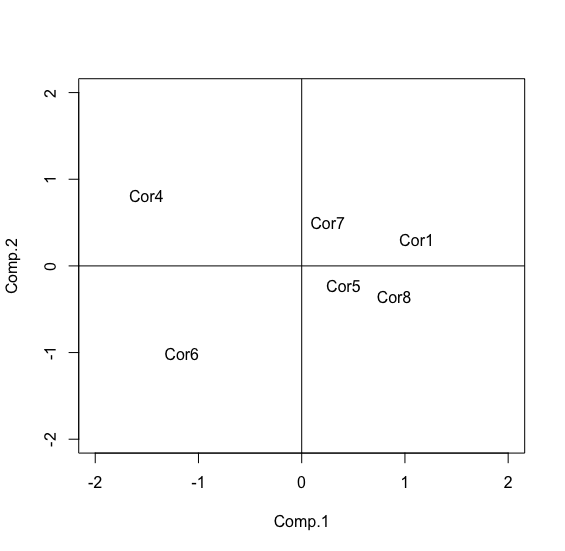
\includegraphics[width=.3\linewidth]{img/2-1-2-individus-premier-plan-factoriel}
	\caption{\scriptsize Individus (correcteurs) dans le premier plan factoriel de l'ACP}
	\label{fig:individus_premier_plan_factoriel}
\end{figure}


\subsection{Représentation des variables d'origine dans le premier plan factoriel}

Afin de représenter les variables d'origine dans le premier plan factoriel, on va tout d'abord calculer leur corrélation. C'est à dire calculer une mesure de la représentation des variables d'origine par les nouveaux axes trouvés à l'aide de l'ACP. Si par exemple la première variable a une corrélation égale à $|1|$ avec le premier axe factoriel, alors ils représentent exactement la même chose. Si à l'inverse la corrélation vaut $0$, on pourra dire que cette variable ne s'exprime absolument pas sur le premier axe factoriel.

On calcule la matrice de corrélation à l'aide de la fonction \texttt{cor} de R~:
\begin{table}[ht]
	\centering
	\begin{tabular}{r|rrrr}
		& Comp.1 & Comp.2 & Comp.3 & Comp.4 \\ 
		\hline
		moy.median & -0.08 & -0.93 & -0.15 & 0.33 \\ 
		std.median & 0.57 & -0.76 & -0.05 & -0.31 \\ 
		moy.final & -0.99 & -0.11 & -0.01 & -0.06 \\ 
		std.final & -0.00 & -0.46 & 0.89 & 0.06 \\ 
	\end{tabular}
\end{table}

On reporte maintenant ces mesures sur le premier plan factoriel afin de représenter les variables d'origine sur ce dernier~:
\begin{figure}[H]
	\centering
	\captionsetup{justification=centering, margin=2cm}
	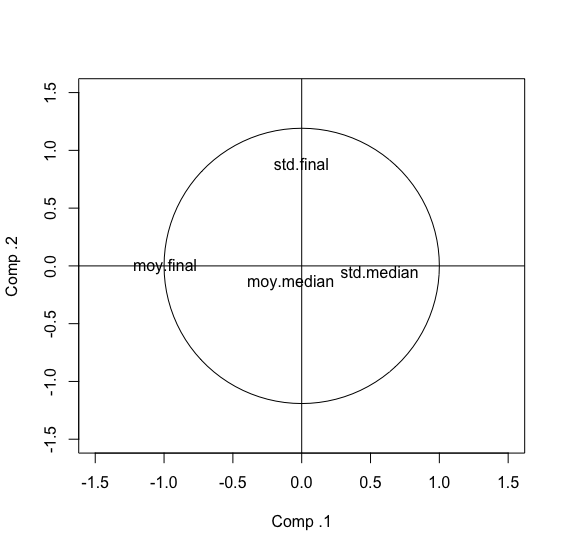
\includegraphics[width=.5\linewidth]{img/2-1-2-variables-premier-plan-factoriel}
	\caption{\scriptsize Variables dans le premier plan factoriel de l'ACP}
	\label{fig:variables_premier_plan_factoriel}
\end{figure}



\subsection{Reconstitution de la matrice originelle \textit{X} centrée en colonne}

On obtient $C$ avec la formule $C = XMU$ ($X$ matrice des observations centrées en colonne, $M = I_p$ et $U$ matrice des vecteurs propres représentant les axes factoriels obtenus après ACP).
\begin{align*}
C &= XMU \\
\Longleftrightarrow \quad CU^T &= XMUU^T \qquad or\ MUU^T = I_p \\
\Longleftrightarrow \quad CU^T &= X
\end{align*}



La somme $\sum\limits_{\alpha=1}^k = c_\alpha u_{\alpha}^T$ est donc égale à une approximation de la matrice centrée en colonne $X$ d'origine, exprimée en fonction des $\alpha$ premiers axes factoriels de l'ACP. Pour $\alpha = k$, donc en prenant en compte 100\% de l'inertie expliquée, on obtient la matrice $X$ (centrée en colonne) d'origine.



\subsection{Représenter les individus possédant des valeurs manquantes}

Nous allons représenter les individus possédant des valeurs manquantes avec la méthode d'imputation par la moyenne~: chaque valeur non renseignée sera remplacée par la moyenne de la variable correspondante.

L'ACP effectuée avec la fonction \texttt{princomp} donne la représentation suivante des individus sur le premier plan factoriel~:

\begin{figure}[H]
	\centering
	\captionsetup{justification=centering, margin=4cm}
	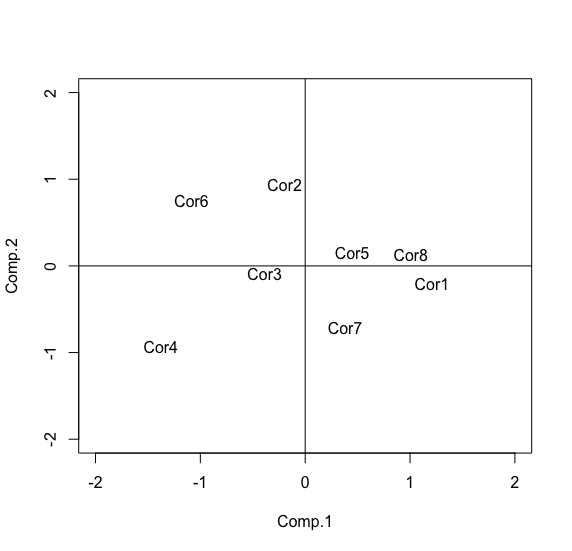
\includegraphics[width=.3\linewidth]{img/2-1-5-individus-with-na-premier-plan-factoriel}
	\caption{\scriptsize Individus (dont les correcteurs 2 et 3 précédemment supprimés) dans le premier plan factoriel de l'ACP}
	\label{fig:individus_with_na_premier_plan_factoriel}
\end{figure}


\section{Utilisation des outils R}

L'objectif est de se familiariser avec les fonctions de R permettant d'effectuer une ACP en utilisant le jeu de données de notes du polycopié de cours. Ce jeu de données contient les notes de neuf élèves dans les matières mathématique, sciences, français, latin et dessin.


\subsection{ACP avec la fonction \texttt{princomp}}

En effectuant l'ACP avec la fonction \texttt{princomp}, on obtient un objet de type \texttt{princomp} qui possède plusieurs attributs nous permettant de retrouver les différentes parties d'une ACP.

\begin{itemize}
	\item \textbf{valeurs propres}~: correspond à l'attribut \texttt{\$sdev}, les écart types de chaque composante.
	\item \textbf{vecteurs propres}~: correspond à l'attribut \texttt{\$loadings}.
	\item \textbf{composantes principales}~: correspond à l'attribut \texttt{\$scores}.
\end{itemize}

Appeler la méthode \texttt{summary} sur le résultat de l'ACP (voir \autoref{fig:2-2-2-summary-acp}) donne l'inertie expliquée de chacune des composantes, ainsi que leur pourcentage simple et cumulé.

\begin{figure}[H]
	\centering
	\captionsetup{justification=centering, margin=2cm}
	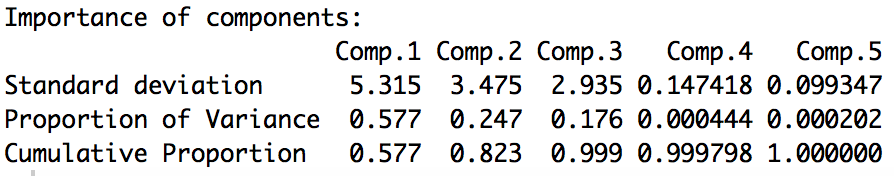
\includegraphics[width=.5\linewidth]{img/2-2-2-summary-acp}
	\caption{\scriptsize Résultat de \texttt{summary} sur l'objet d'ACP retourné par la fonction \texttt{princomp}}
	\label{fig:2-2-2-summary-acp}
\end{figure}

\subsection{ACP~: fonctions \texttt{plot} et \texttt{biplot}}

La fonction \texttt{plot} permet de représenter les résultats de l'ACP de différentes façon. Appeler \texttt{plot} sur l'objet ACP donne les pourcentages de variance pour chaque composante (voir \autoref{fig:2-2-2-plot-acp}). Si on appelle la méthode sur \texttt{ACP\$scores} alors on obtiendra la représentation des individus dans le premier plan factoriel (voir \autoref{fig:2-2-2-plot-acp-scores}). Si on veux utiliser d'autres composantes, il faudra le spécifier directement en choisissant les colonnes à utiliser dans la matrice des composantes principales. Et enfin, si on appelle \texttt{plot} sur \texttt{ACP\$loadings} on obtiendra la représentation des variables d'origine sur le premier plan factoriel (voir \autoref{fig:2-2-2-plot-acp-loadings}).

\begin{figure}[H]
	\centering
	\captionsetup{justification=centering, margin=2cm}
	\begin{subfigure}[b]{0.28\linewidth}
		\centering
		\captionsetup{justification=centering}
		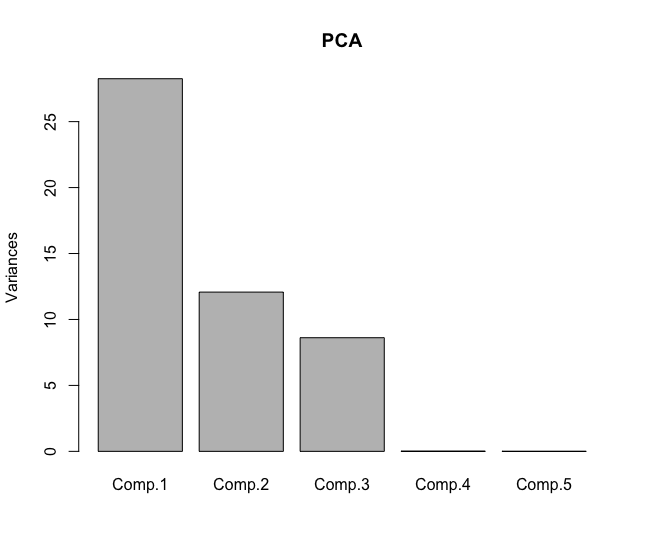
\includegraphics[width=1\linewidth]{img/2-2-2-plot-acp}
		\caption{\scriptsize Pourcentages de variance pour chaque composante.}
		\label{fig:2-2-2-plot-acp}
	\end{subfigure}%
	\begin{subfigure}[b]{0.28\linewidth}
		\centering
		\captionsetup{justification=centering}
		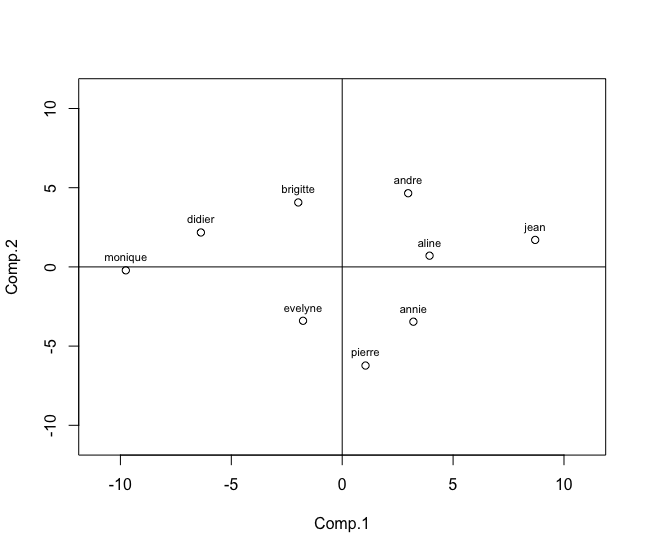
\includegraphics[width=1\linewidth]{img/2-2-2-plot-acp-scores}
		\caption{\scriptsize Individus sur le premier plan factoriel.}
		\label{fig:2-2-2-plot-acp-scores}
	\end{subfigure}%
	\begin{subfigure}[b]{0.28\linewidth}
		\centering
		\captionsetup{justification=centering}
		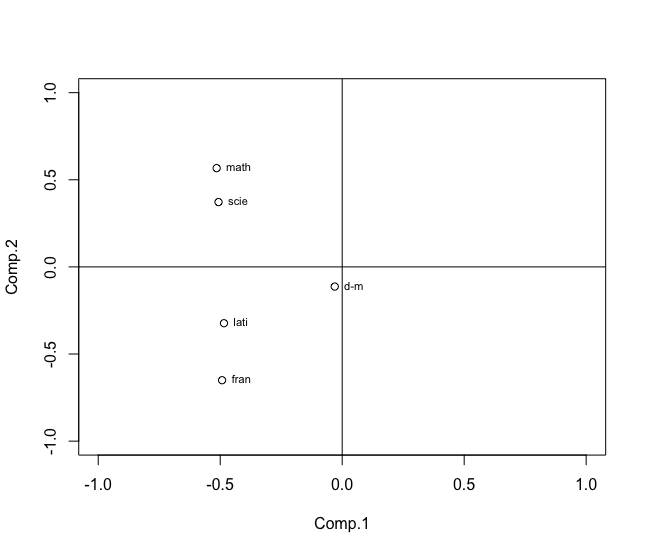
\includegraphics[width=1\linewidth]{img/2-2-2-plot-acp-loadings}
		\caption{\scriptsize Variables d'origine sur le premier plan factoriel.}
		\label{fig:2-2-2-plot-acp-loadings}
	\end{subfigure}%
	\caption{Résultats de la fonction \texttt{plot}.}
\end{figure}



La fonction \texttt{biplot} redéfinie pour l'ACP va mélanger les deux représentations sur le premier plan factoriel (par défaut)~: on aura les individus ainsi que l'expression de la corrélation entre les variables d'origine et les composantes principales (voir \autoref{fig:2-2-2-biplot-acp}).

\begin{figure}[H]
	\centering
	\captionsetup{justification=centering, margin=1cm}
	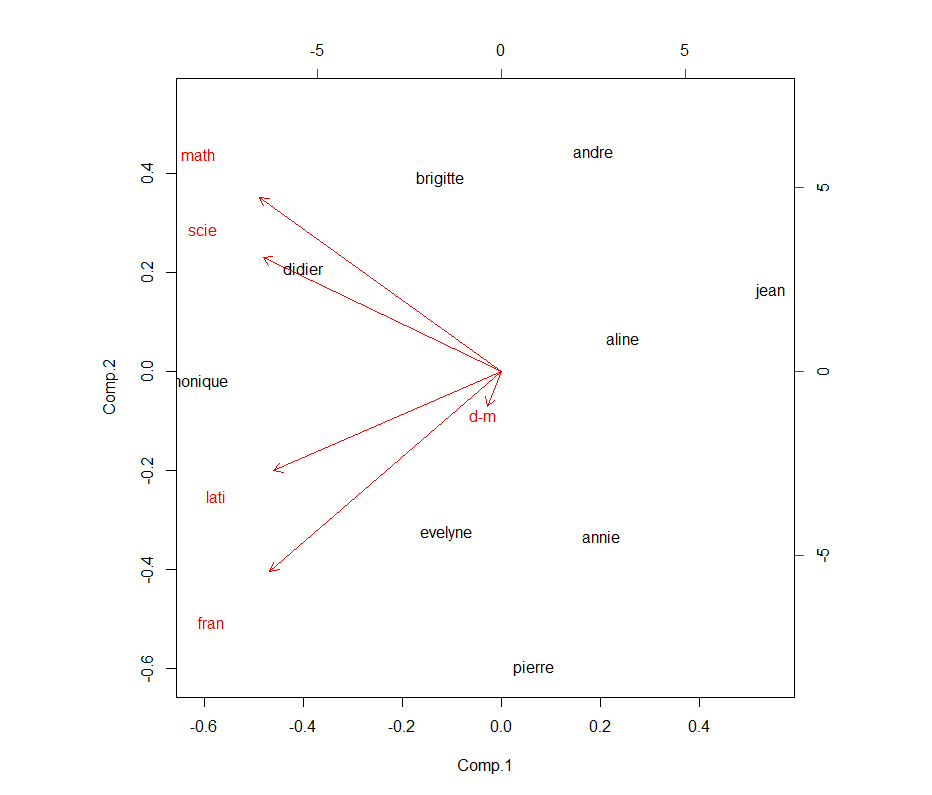
\includegraphics[width=.5\linewidth]{img/2-2-2-biplot-composante-1-2}
	\caption{\scriptsize Biplot par défaut sur le premier plan factoriel.}
	\label{fig:2-2-2-biplot-acp}
\end{figure}

On remarque qu'il y a deux échelles de valeur pour chaque axe (haut et bas pour \textit{Comp.1} et gauche et droite pour \textit{Comp.2}). Les axes bas et gauche mesurent la corrélation entre les variables d'origine et les nouveaux axes factoriels. Les axes haut et droit mesurent les valeurs prises par les individus dans le premier plan factoriel.

Options de la fonction \texttt{biplot}~:
\begin{itemize}
	\item \textbf{choices}~: un vecteur de longueur 2 spécifiant les composantes à utiliser. Par défaut ce sont les deux premières qui sont choisies
	
	\item \textbf{scale}~: réel comprit entre 0 et 1, permet d'adapter l'échelle des représentations entre les individus et les variables
	\begin{itemize}
		\item Les variables sont mise à l'échelle par $\lambda^{scale}$
		\item Les observations sont mise à l'échelle par $\lambda^{1-scale}$
		\item $\lambda$ représente les valeurs propres calculées par l'ACP
	\end{itemize}

	\item \textbf{pc.biplot}~: booléen, si \textit{vrai} utilise la représentation de Gabriel (1971)
	\begin{itemize}
		\item Les observations sont mises à l'échelle par $\sqrt{n}$ ($n$ est la taille de l'échantillon)
		\item Alors le produit interne entre les variables donne une approximation des covariances et les distance entre les observations donnent une approximation de la distance de Mahalanobis
	\end{itemize}
\end{itemize}

\section{Données Crabs}
\label{sec:2_3_ACP_Crabs}

\subsection{ACP sur les données initiales}

Voici ci-dessous un tableau récapitulatif de l'ACP effectuée sur les données \texttt{crabsquant} sans traitement préalable.

\begin{table}[H]
	\centering
	\captionsetup{justification=centering, margin=2cm}
	\caption{ACP sur le jeu de données "crabs" (sans traitement préalable)}
	\label{table:acp_crabs_initial_data}
	\begin{tabular}{lrrrrr}
		& Comp. 1 & Comp. 2 & Comp. 3 & Comp. 4 & Comp. 5 \\
		Inertie expliquée & 11.83 & 1.14 & 1 & 0.37 & 0.28 \\
		Pourcentage d'inertie expliquée & 98.25 & 0.91 & 0.70 & 0.09 & 0.05 \\
		Pourcentage d'inertie expliquée cumulé & 98.25 & 99.16 & 99.86 & 99.95 & 100
	\end{tabular}
\end{table}

On constate que la première composante représente 98.25\% des données à elle toute seule. Si on calcule la matrice de corrélation entre les nouvelles composantes principales et les variables d'origine (\autoref{table:correlation_crabs_acp}), on remarque alors que toutes les variables d'origine sont très fortement corrélées à la première composante principale.
Tout particulièrement les variables \textit{CL} et \textit{CW}, c'est à dire la longueur et la largeur de la coquille des crabes.

\begin{table}[H]
	\centering
	\captionsetup{justification=centering, margin=2cm}
	\caption{Corrélations entre les variables d'origines et les composantes principales (données "crabs")}
	\label{table:correlation_crabs_acp}
	\begin{tabular}{r|rrrrr}
		& Comp.1 & Comp.2 & Comp.3 & Comp.4 & Comp.5 \\ 
		\hline
		FL & -0.981 & -0.105 & 0.145 & 0.077 & 0.010 \\ 
		RW & -0.909 & -0.383 & -0.161 & -0.021 & -0.015 \\ 
		CL & -0.999 & 0.032 & 0.025 & -0.007 & -0.029 \\ 
		CW & -0.997 & 0.042 & -0.062 & 0.006 & 0.017 \\ 
		BD & -0.983 & -0.053 & 0.160 & -0.068 & 0.036 \\ 
	\end{tabular}
\end{table}

On retrouve bien ici l'effet de taille observé précédemment dans la  \autoref{subsection:crabs_correlation_variables_quantitatives}. La représentation graphique de l'ACP obtenue avec la commande \texttt{biplot} (\autoref{fig:biplot_acp_crabs_plan_1_2}) confirme cette corrélation~: les variables \textit{CW} et \textit{CL} sont particulièrement bien exprimée par le premier axe factoriel, tout comme \textit{BD} et \textit{FL}. Seule la mesure \textit{RW} "s'émancipe" un peu est s'exprime légèrement sur le second axe factoriel.\\
Une rapide analyse du tableau de corrélation (\autoref{table:correlation_crabs_acp}) nous indique d'ailleurs que les composantes 2 et 3 pourraient bien mieux représenter les variables \textit{FL}, \textit{RW} et \textit{BD}. Et effectivement, une représentation des individus sur le plan factoriel créé à partir du deuxième et troisième axe (\autoref{fig:biplot_acp_crabs_plan_2_3}), permet à priori de mieux discriminer la population de crabes selon leur espèce et leur sexe. Mais il ne faut pas oublier qu'en ne considérant pas la premier axe factoriel, on perd 98\% de l'inertie expliquée...

\begin{figure}[H]
	\centering
	\captionsetup{justification=centering, margin=2cm}
	\begin{subfigure}[b]{0.5\linewidth}
		\centering
		\captionsetup{justification=centering, margin=1cm}
		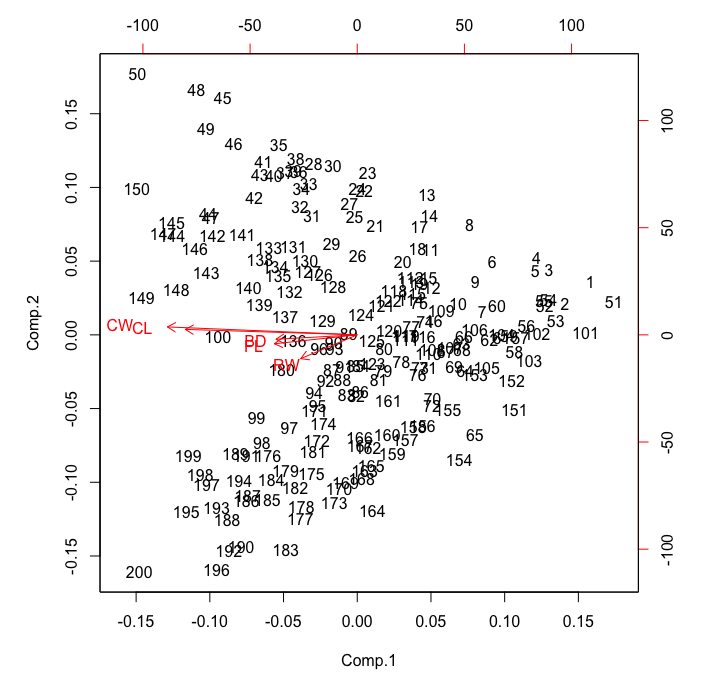
\includegraphics[width=1\columnwidth]{img/2-3-1-biplot-acp-crabs-plan-1-2}
		\caption{\scriptsize ACP crabs~: biplot du premier \\plan factoriel}
		\label{fig:biplot_acp_crabs_plan_1_2}
	\end{subfigure}%
	\begin{subfigure}[b]{0.5\linewidth}
		\centering
		\captionsetup{justification=centering, margin=1cm}
		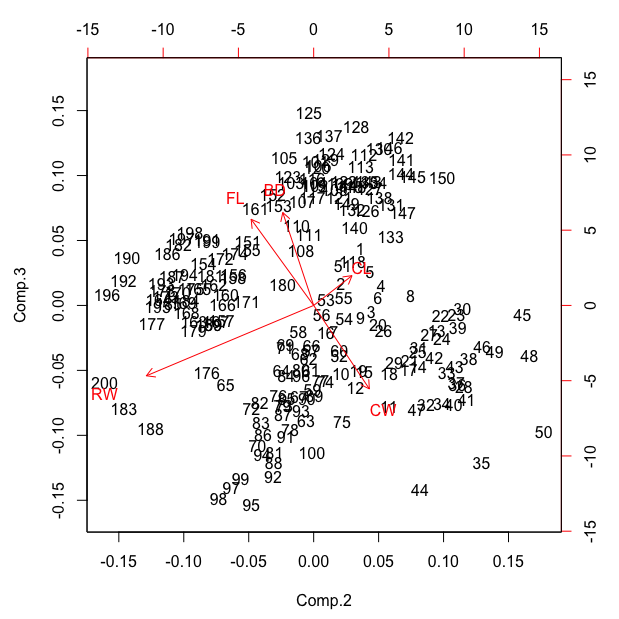
\includegraphics[width=1\columnwidth]{img/2-3-1-biplot-acp-crabs-plan-2-3}
		\caption{\scriptsize ACP crabs~: biplot du plan factoriel créé à partir des composantes 2 et 3}
		\label{fig:biplot_acp_crabs_plan_2_3}
	\end{subfigure}%
	\caption{
		\small Représentations de l'ACP des données \texttt{crabs} sur deux plans factoriels différents
	}
	\label{fig:biplots_crabs}%
\end{figure}



\subsection{Correction de l'effet de taille}

Afin de prendre en compte une plus grande partie de l'inertie expliquée, il va nous falloir corriger l'effet de taille. Le principe de l'ACP est d'identifier les axes présentant la plus grande dispersion possible, et l'ACP précédente a bien montré que la taille du crabe est le facteur le plus "dispersant". Il va donc falloir réduire au maximum cette dispersion afin donner plus d'importance aux autres mesures et peut-être identifier des facteurs morphologiques (autres que la taille) communs au sexe et/ou aux espèces.\\
On a identifié les variables \textit{CL} et \textit{CW} comme étant les initiatrices principales de cet effet de taille. Il suffit alors de réduire à 0 la dispersion de l'une de ces deux mesures. Une manière simple de faire cela est d'exprimer l'ensemble des autres variables en pourcentage de la mesure dont on veut réduire la dispersion. Nous avons ici choisit de réduire la dispersion de la mesure \textit{CL} (les effets de \textit{CL} et \textit{CW} sur l'ACP sont quasiment identiques, donc ici choisir l'une ou l'autre revient finalement au même, comme on peut le voir dans la \autoref{fig:biplot_acp_crabs_corrected_CW}).\\
La méthode est donc, pour chaque individu, de diviser toutes les observations par la valeur de \textit{CL} puis de multiplier par 100. Le \autoref{table:comparatif_normalisation_crabs} montre bien le changement se produisant dans les observations.

\begin{table}[H]
	\centering
	\captionsetup{justification=centering, margin=4cm}
	\caption{\scriptsize Comparatif des observations du premier individu avant et après correction de l'effet de taille}
	\label{table:comparatif_normalisation_crabs}
	\begin{tabular}{r|rrrrr}
		& FL & RW & CL & CW & BD \\ 
		\hline
		Avant correction & 8.10 & 6.70 & 16.10 & 19.00 & 7.00 \\ 
		Après correction & 50.31 & 41.61 & 100.00 & 118.01 & 43.48 \\ 
	\end{tabular}
\end{table}

Tous les individus auront donc maintenant une valeur de 100 pour la variable \textit{CL}~: sa dispersion sera nulle. L'ACP effectuée sur les nouvelles données ainsi corrigée (\autoref{table:acp_crabs_corrected_data}) est bien plus "équilibrée" dans le sens où la première composante principale ne représente pas 98\% des données mais 53\%, et qu'il faut prendre en compte les 3 premiers axes factoriels pour obtenir environ 95\% d'inertie expliquée.



\begin{table}[H]
	\centering
	\captionsetup{justification=centering, margin=2cm}
	\caption{ACP sur le jeu de données \texttt{crabs} \\(avec correction de l'effet de taille)}
	\label{table:acp_crabs_corrected_data}
	\begin{tabular}{lrrrrr}
		& Comp. 1 & Comp. 2 & Comp. 3 & Comp. 4 & Comp. 5 \\
		Inertie expliquée & 3.936 & 3.217 & 1.333 & 1.2302 & 0 \\
		Pourcentage d'inertie expliquée & 53.2 & 35.5 & 6.1 & 5.19 & 0 \\
		Pourcentage d'inertie expliquée cumulé & 53.2 & 88.7 & 94.8 & 100 & 100
	\end{tabular}
\end{table}



Voici la représentation des données sur le nouveau plan factoriel déterminé par l'ACP. On remarque une séparation très claire du sexe et de l'espèce avec la formation de quatre grappes de points bien séparées.


\begin{figure}[H]
	\centering
	\captionsetup{justification=centering, margin=2cm}
	\begin{subfigure}[b]{0.5\linewidth}
		\centering
		\captionsetup{justification=centering, margin=1cm}
		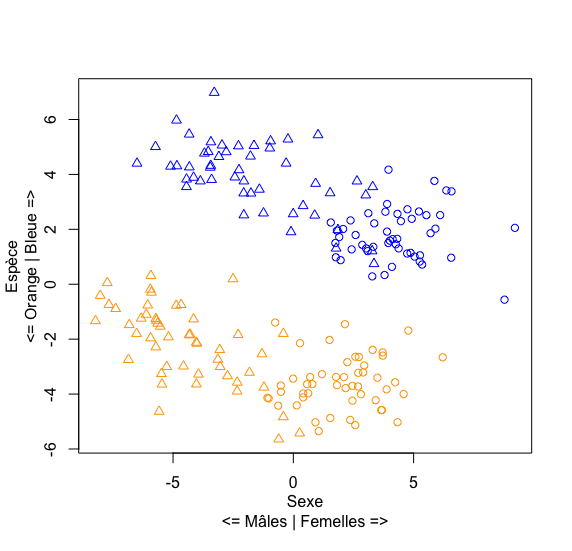
\includegraphics[width=1\columnwidth]{img/2-3-2-biplot-acp-crabs-corrected-CL}
		\caption{\scriptsize ACP crabs~: correction de l'effet de taille en normalisant par rapport à la variable \textit{CL}}
		\label{fig:biplot_acp_crabs_corrected_CL}
	\end{subfigure}%
	\begin{subfigure}[b]{0.5\linewidth}
		\centering
		\captionsetup{justification=centering, margin=1cm}
		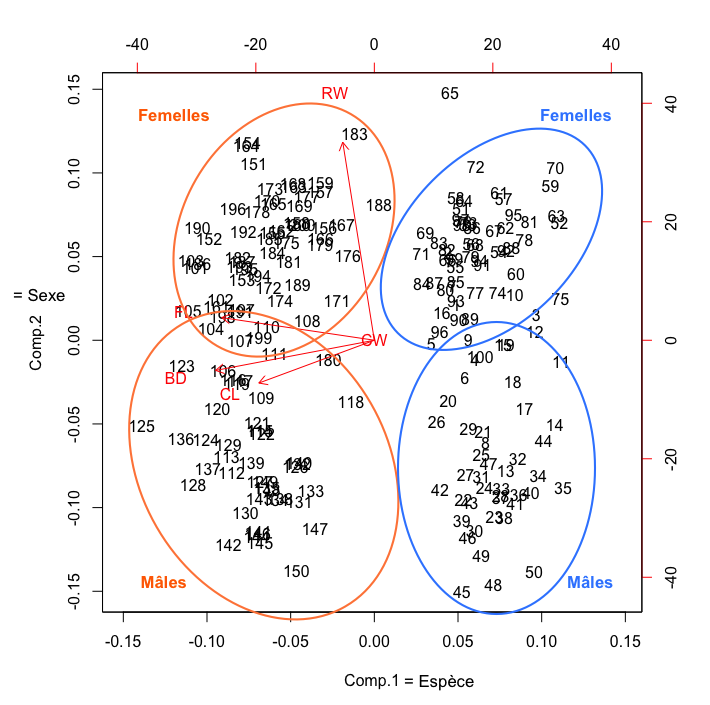
\includegraphics[width=1\columnwidth]{img/2-3-2-biplot-acp-crabs-corrected-CW}
		\caption{\scriptsize ACP crabs~: correction de l'effet de taille en normalisant par rapport à la variable \textit{CW}}
		\label{fig:biplot_acp_crabs_corrected_CW}
	\end{subfigure}%
	\caption{
		\small Représentations de l'ACP des données \texttt{crabs} après correction de l'effet de taille
	}
	\label{fig:biplots_crabs_corrected}%
\end{figure}

La coloration (bleue ou orange) et la différenciation du type de point (triangle pour les mâles, rond pour les femelles) nous a permis d'identifier la signification des axes du premier plan factoriel~: sexe et espèce. Remarquons que choisir \textit{CL} ou \textit{CW} comme base pour la normalisation des observation va simplement inverser les deux premiers axes factoriels.


Conclusion~: la suppression de l'effet de taille permet de véritablement discriminer les observations en fonction de l'espèce et du sexe des individus, et non plus seulement en fonction de leur taille.

\section{Données Pima}
\label{sec:2_4_ACP_Pima}


On effectue l'analyse en composantes principales sur les variables quantitatives du jeu de données \texttt{Pima} et on obtient les résultats suivants.

\begin{figure}[H]
	\centering
	\captionsetup{justification=centering, margin=1cm}
	\begin{subfigure}[b]{0.45\linewidth}
		\centering
		\captionsetup{justification=centering, margin=0cm}
		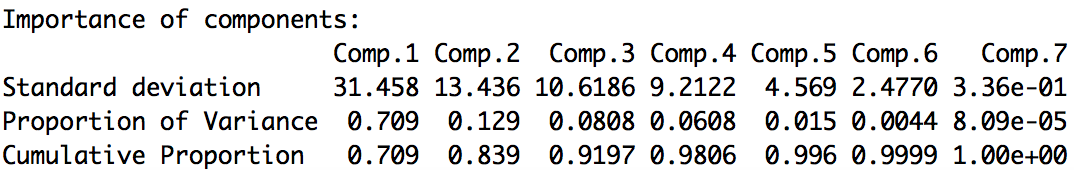
\includegraphics[width=1\columnwidth]{img/2-4-ACP-Pima-Pourcentage-Inertie-Expliquee}
		\caption{\scriptsize ACP \texttt{Pima}~: Pourcentage d'inertie expliquée}
		\label{fig:2-4-ACP-Pima-Pourcentage-Inertie-Expliquee}
	\end{subfigure}%
	\begin{subfigure}[b]{0.45\linewidth}
		\centering
		\captionsetup{justification=centering, margin=0cm}
		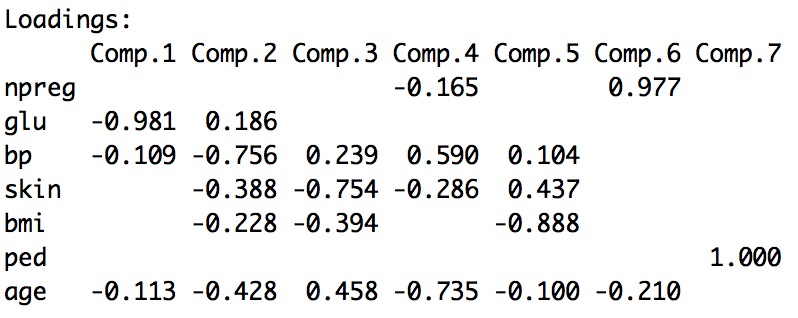
\includegraphics[width=.8\columnwidth]{img/2-4-ACP-Pima-Axes-Factoriels}
		\caption{\scriptsize ACP \texttt{Pima}~: Axes factoriels (vecteurs propres résultants de l'ACP)}
		\label{fig:2-4-ACP-Pima-Axes-Factoriels}
	\end{subfigure}%
	\caption{
		\small ACP sur \texttt{Pima}~: inertie expliquée et axes factoriels.
	}
	\label{fig:ACP-Pima-inertie-et-axes-factoriels}%
\end{figure}




\begin{table}[H]
	\centering
	\captionsetup{justification=centering, margin=2cm}
	\caption{ACP sur \texttt{Pima}~: corrélation entre les variables d'origine et les nouveaux axes factoriels.}
	\begin{tabular}{r|rrrrrrr}
		& Comp.1 & Comp.2 & Comp.3 & Comp.4 & Comp.5 & Comp.6 & Comp.7 \\ 
		\hline
		npreg & -0.16 & -0.36 & 0.32 & -0.46 & 0.01 & 0.73 & 0.00 \\ 
		glu & -1.00 & 0.08 & 0.01 & 0.01 & 0.00 & 0.00 & -0.00 \\ 
		bp & -0.28 & -0.83 & 0.21 & 0.44 & 0.04 & 0.00 & 0.00 \\ 
		skin & -0.27 & -0.50 & -0.76 & -0.25 & 0.19 & -0.00 & -0.00 \\ 
		bmi & -0.29 & -0.45 & -0.61 & 0.02 & -0.59 & 0.01 & -0.00 \\ 
		ped & -0.17 & -0.01 & -0.08 & -0.07 & -0.08 & -0.04 & 0.98 \\ 
		age & -0.33 & -0.53 & 0.45 & -0.63 & -0.04 & -0.05 & -0.00 \\ 
	\end{tabular}
	\label{table:correlation-acp-pima}
\end{table}

On voit que le premier plan factoriel représente environ 83\% de l'inertie expliquée, ce qui est encourageant.
Par contre, on remarque aussi que les axes factoriels semblent être particulièrement représentatifs de certaines variables d'origine. Et c'est confirmé par la matrice de corrélation entre les variables d'origine et les nouveaux axes factoriels (voir \autoref{table:correlation-acp-pima}). Le premier axe factoriel est quasiment équivalent à la variable \texttt{glu}, le second à la variable \texttt{bp}, le troisième représente plutôt les variables \texttt{skin} et \texttt{bmi}, le quatrième l'âge, le cinquième \texttt{bmi} encore et le sixième le nombre de grossesses. Le septième axe est le plus flagrant d'entre tous~: il est quasiment équivalent à la variable \texttt{ped} d'origine.

L'ACP n'est pas concluante. Les sept composantes principales trouvées sont un reflet trop proche des sept variables initiales. Une représentation graphique des observations sur le premier plan factoriel ne permet pas de distinguer visuellement les groupes de patientes diabétiques et non diabétiques.


\begin{figure}[H]
	\centering
	\captionsetup{justification=centering, margin=2cm}
	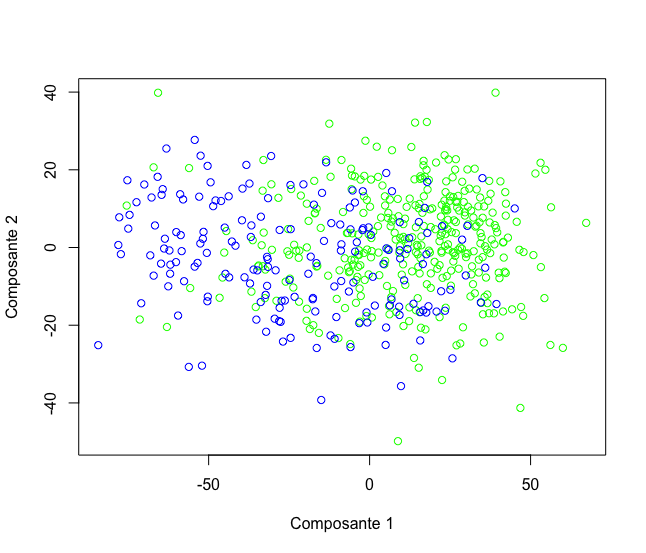
\includegraphics[width=.4\linewidth]{img/2-4-Pima-ACP-premier-plan-factoriel}
	\caption{\scriptsize Représentation des données \texttt{Pima} sur le premier plan factoriel.\\ \tiny Rappel~: bleu pour diabétique, vert pour non diabétique}
	\label{fig:2-4-Pima-ACP-premier-plan-factoriel}
\end{figure}


Nous avons fait une nouvelle ACP en changeant la matrice $D_p$ de poids des individus, en spécifiant que le poids d'un individu d'un groupe $g$ valait $\frac{1}{card(g)}$, afin de rééquilibrer le poids de chaque groupe.

\begin{figure}[H]
	\centering
	\captionsetup{justification=centering, margin=2cm}
	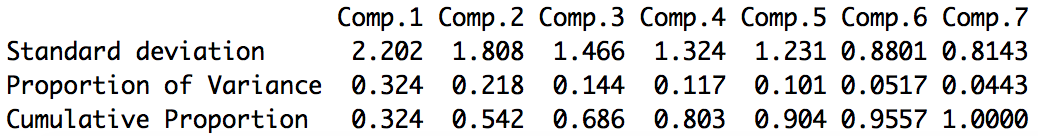
\includegraphics[width=.7\linewidth]{img/2-4-Pima-ACP-dp-inertie-expliquee}
	\caption{\scriptsize Inertie expliquée de l'ACP avec poids des individus normalisé en fonction de leur groupe}
	\label{fig:2-4-Pima-ACP-dp-inertie-expliquee}
\end{figure}

On obtient la table de corrélation suivante entre les variables d'origine est les nouvelles composantes principales~:

\begin{table}[H]
	\centering
	\captionsetup{justification=centering, margin=2cm}
	\caption{ACP après modification du poids des individus: corrélation entre les variables d'origine et les nouveaux axes factoriels.}
	\begin{tabular}{r|rrrrrrr}
		& Comp.1 & Comp.2 & Comp.3 & Comp.4 & Comp.5 & Comp.6 & Comp.7 \\ 
		\hline
		npreg & -0.54 & 0.67 & -0.01 & -0.28 & 0.20 & 0.26 & 0.16 \\ 
		glu & -0.58 & -0.10 & -0.23 & 0.71 & 0.18 & 0.08 & 0.06 \\ 
		bp & -0.60 & 0.05 & 0.37 & 0.11 & -0.70 & -0.01 & 0.15 \\ 
		skin & -0.64 & -0.51 & 0.27 & -0.29 & 0.30 & -0.29 & 0.24 \\ 
		bmi & -0.62 & -0.61 & 0.27 & -0.20 & 0.07 & 0.28 & -0.32 \\ 
		ped & -0.27 & -0.27 & -0.83 & -0.26 & -0.25 & -0.01 & 0.03 \\ 
		age & -0.68 & 0.58 & -0.04 & -0.07 & 0.03 & -0.35 & -0.31 \\ 
	\end{tabular}
\end{table}

On remarque que la première composante principale est maintenant corrélée avec toutes les variables d'origine ou presque, la deuxième aussi et la troisièmes dans une moindre mesure.

Au final, ce traitement des données ne change pas grand chose, les classes ne permettent pas de bien différencier les groupes de femmes diabétiques et non diabétiques.


Peut-être serait-il plus pertinent de changer le poids des variables, et d'attribuer plus de poids à celles dont on a vu dans l'analyse descriptive (voir \autoref{section:pima-descriptif}) qu'elles ont un lien fort avec le facteur diabète.

\end{document}
